\documentclass[main.tex]{subfiles}

\begin{document}

\chapter{Pione: lightest meson}

\section{Risultati sperimentali}

\subsection{Energia cinetica dei frammenti di un decadimento}
$\underbrace{A}_M\rightarrow \underbrace{a_1}_{m_1}+\underbrace{a_2}_{m_2}$, nel riferimento di quiete di CM.

\begin{align*}
&M=m_1+m_2+T_1+T_2=e_1+e_2 & \intertext{questa sopra \'e la conservazione dell'energia (c=1)}\\
&0=\vec{p_1}+\vec{p_2}\\
&\underbrace{\vec{p_1}^2}_{e_1^2-m_1^2}=\underbrace{\vec{p_2}^2}_{e_2^2-m_2^2} & \intertext{questa ultima sopra la conservazione dell'impulso (CM)}\\
&M=e_1+e_2\\
&e_1=\frac{M^2+m_1^2-m_2^2}{2M}\\
&e_2=\frac{M^2+m_2^2-m_1^2}{2M}
\end{align*}

\subsection{Tipo di interazione}
Interaction: Strong.

\'E un mesone.

\subsection{Tripleto di isospin.}
Isospin $T=1$: 3 stati di una stessa particella con Isospin $T=1$.

\begin{tabular}{|l|lll|}
\hline
&\Ppiplus&\Ppizero&\Ppiminus\\
\hline
$T_3$&-1&0&1\\
\hline
\end{tabular}\\

\Ppipm sono reciprocamente antiparticelle, \Ppizero \'e l'antiparticella di se stessa.

\subsection{ Massa}
$m_{\Ppizero}=135 \Mcs$, $m_{\Ppipm}=139.5\Mcs$.

La differenza di massa pu\'o essere attribuita alla non conservazione dell'isospin nelle interazioni EM.

\subsection{Metodi misura massa pione}
\begin{itemize*}
\item \Ppiminus\\
radiazione X atomo $\pi$-mesico.

Livelli atomo pionico:

\begin{align*}
&E_n^{\Ppiminus}=-\frac{1}{4\pi\epsilon_0}\ER^{\Ppiminus}\frac{Z^2}{n^2}=-\frac{m_{\pi}}{m_e}\ER\frac{Z^2}{n^2}\\
&=-\frac{1}{278}\ER\frac{Z^2}{n^2}
\end{align*}
\index{Livelli atomo pionico}

\item \Ppiplus\\
Dalla reazione $\Ppiplus\rightarrow\APmuon+\Pnum$.

\item \Ppizero\\
Dalla reazione $\Ppizero\rightarrow2\gamma$.

\end{itemize*}

\subsection{Spin e parit\'a}
$S=0$ \'e un bosone. Parit\'a: $\Pi_{\pi}=-1$.

\subsection{Composizione}

\begin{tabular}{|l|l|l|}
\Ppiplus&\Ppizero&\Ppiminus\\
\Pup\APdown&\Pup\APup or \Pdown\APdown&\Pdown\APup\\
\end{tabular}

\section{Modi di decadimento}

\subsection{Modi decadimento pioni}
\Ppizero:

\begin{enumerate*}
\item $\Ppizero\rightarrow\gamma+\gamma$ ($98.8\%$) (Lo spin del pione \'e intero:) $\tau_{\Ppizero}\approx10^{-16} s$.
\item Decadimento di Dalitz:

$\Ppizero\rightarrow\gamma+\Pelectron+\APelectron$ ($1.2\%$).
\end{enumerate*}

\Ppiminus:

\begin{enumerate*}
\item $\Ppiminus\rightarrow\Pmuon+\APnum$ ($100\%$) (J=S+L) Lo spin finale=0,1: Lo spin del pione \'e intero.

$\tau_{\Ppiminus}\approx10^{-8}$
\end{enumerate*}

\Ppiplus:

\begin{enumerate*}
\item $\Ppiplus\rightarrow\APmuon+\Pnum$ ($100\%$)\\
$\tau_{\Ppiplus}=
10^{-8}$
\end{enumerate*}

\subsection{Branching ratio: densit\'a stati finali}
Il decadimento dei \Ppiminus \'e quasi essenzialmente $\Ppiminus\to\Pmuon+\APnum$: il decadimento $\Ppiminus\to\Pelectron+\APnue$ \'e fortemente inibito.

Si ha che $\lambda=\frac{1}{\tau}\propto|M_{if}|^2\rho(E_f)$ cio\'e, assumendo che $|M_{if}^e|^2\approx |M_{if}^{\mu}|^2$, la differente densit\'a di stati finali spiega la differenza di probabilit\'a:

\begin{align*}
\rho(E_f)=\frac{1}{V}\frac{\,dn}{dE_f}=\frac{4\pi p^2}{h^3}\frac{dp}{dE_f}\\
E_f=E_{\nu}+E_{\Pl}=cp+\sqrt{c^2p^2+m^2c^4}&\intertext{per decadimenti in quite i moduli dei momenti dei prodotti sono uguali e opposti: $|p_{\nu}|=|p_{\Pl}|$}
\end{align*}


Il momento angolare si conserva quindi gli spin, dato che il pione ha spin 0, gli spin dei prodotti sono opposti: i neutrini hanno spin e momento paralleli e, per la conservazione del momento angolare, ci\'o deve essere per l'elettrone.

Helicity in beta decay.

Gli elettroni nel beta decay hanno $h=\frac{\scap{s}{J}}{|\scap{s}{p}|}=-\frac{v}{c}\approx-1$ per gli elettroni ultrarelativistici emessi nel decadimento del pione.

La frazione di elettroni con elicit\'a positiva \'e
\begin{equation*}
1-\frac{v}{c}=\frac{2m^2}{m_{\pi}^2+m^2}\quad\text{m=massa leptone carico}
\end{equation*}
e la probabilit\'a di decadimento \'e inibita dello stesso fattore.

\subsection{Helicity: Massless vs massive particles.}
If electrons and muon were massless two body pion decay would be forbidden: they would have $100\%$ right-hand chirality.

Because of their finite mass electrons and muons with their spins pointing in their direction of motion also have a left-handed component.

\section{Misura dello spin e della parit\'a del pione}

\subsection{Sezione d'urto e Regola d'oro di Fermi}

\begin{equation*}
\frac{\# \text{Transizioni}}{\text{Tempo}}=w=\frac{2\pi}{\hbar}|\braket{\psi_{Bb}|H|\psi_{Aa}}|^2\rho(E)
\end{equation*}
con $\rho(E)=\frac{dn}{dE}=\frac{\# \text{stati finali}}{\text{Unit\'a Energia}}$.

Relazione fra $\sigma(bB\rightarrow aA)$ e $\sigma(aA\rightarrow bB)$ (Invarianza inversione temporale).
\begin{equation*}
\frac{\sigma(aA\rightarrow bB)}{\sigma(bB\rightarrow aA)}=\frac{p_b^2}{p_a^2}\frac{(2s_B+1)(2s_b+1)}{(2s_A+1)(2s_a+1)}
\end{equation*}

Che giustifico: 


Relazione tra la sezione d'urto di una reazione e l'inversa
$a+A\leftrightarrow b+B$.

Particella in valume V:
\begin{align*}
dn=(2s_b+1)(2s_B+1)V\frac{4\pi p_b^2dp_b}{h^3}\\
dE=v_b\,dp_b\\
\end{align*}
e quindi la densit\'a di stati \'e
\begin{equation*}
\frac{dn}{dE}=(2s_b+1)(2s_B+1)V\frac{4\pi p^2}{h^3v_b}
\end{equation*}
e la probabilit\'a di transizione per unit\'a di tempo
\begin{equation*}
w\propto V(2s_b+1)(2s_B+1)\frac{p^2}{h^4v_b}|\braket{\psi_{Bb}|H|\psi_{Aa}}|^2
\end{equation*}
Dalla relazione

\begin{equation*}
N_av_a\sigma(aA\rightarrow bB)=\frac{\# \text{Transizioni}}{\# \parbox{1cm}{Nuclei bersaglio A}*\parbox{1cm}{Unit\'a di tempo}}=w
\end{equation*}

quindi

\begin{equation*}
\sigma(aA\rightarrow bB)\propto V^2\frac{p_b^2}{v_av_b}(2s_b+1)(2s_B+1)|\braket{\psi_{Bb}|H|\psi_{Aa}}|^2
\end{equation*}

Invarianza inversione temporale:

$|\braket{\psi_{Bb}|H|\psi_{Aa}}|^2=|\braket{\psi_{Aa}|H|\psi_{Bb}}|^2$ 
infine ottengo
\begin{equation*}
\frac{\sigma(aA\rightarrow bB)}{\sigma(bB\rightarrow aA)}=\frac{p_b^2}{p_a^2}\frac{(2s_B+1)(2s_b+1)}{(2s_A+1)(2s_a+1)}
\end{equation*}

\subsection{Misura dello spin e della parit\'a del pione.}

Principio del bilancio dettagliato:

Se la natura \'e simmetrica per time reversal, e l'interazione forte lo \'e la sezione d'urto di una reazione e della reazione inversa sono uguali a parte fattori statistici e cinematici.

Il fatto che $H_{fi}$ sia hermitiana implica $\exv{|H_{fi}|^2}=\exv{|H_{if}|^2}$ (i due stati sono calcolati per la stessa energia nel sistema del centro di massa):

$\frac{\sigma_{A\rightarrow B}}{\sigma_{B\rightarrow A}}=\frac{p_b^2(2I_B+1)(2I_b+1)}{p_a^2(2I_A+1)(2I_a+1)}$ le velocit\'a e i momenti sono misurati nel sistema CM.
\index{Principio del bilancio dettagliato}

Studio la reazione $\Pproton+\Pproton\rightarrow d+\Ppiplus$:

Q di reazione:
\begin{equation*}
Q=2m_p-(m_d+m_{\pi})\approx2000MeV-2140Mev<0
\end{equation*}

La reazione non \'e possibile in onda S (a bassa energia).

Determinazione dello spin del pione.

\begin{align*}
\frac{\sigma(pp\to \Ppiplus d)}{\sigma(\Ppiplus d\to pp)}=(\frac{k_{\Ppiplus}}{k_p})^2\frac{(2s_{\Ppiplus}+1)(2s_d+1)}{\frac{1}{2}(2s_p+1)^2}\\
s_p=\frac{1}{2}\quad s_d=1\\
\frac{\sigma(pp\to \Ppiplus d)}{\sigma(\Ppiplus d\to pp)}=\frac{3}{2}(\frac{k_{\Ppiplus}}{k_p})^2(2s_{\Ppiplus}+1)&\intertext{e confronto quest'ultima con i dati sperimentali}
\end{align*}

Ottengo $s_{\pi}=0$.

\subsection{E soglia per creazione particella in bombardamento pp}
\begin{align*}
\Pproton+\Pproton\to\Pproton+\Pproton+X\\
T_{th}=(-Q)\frac{M_i+M_f}{2m_{Target}}
\end{align*}

\subsection{Determinazione della parit\'a del pione}

Considero la reazione
\begin{equation*}
\Ppiminus+D\rightarrow n+n
\end{equation*}

Le interazioni forti conservano la parit\'a e il momento angolare totale:

Conservazione della parit\'a.

\lbt{\Pi_{i}=\Pi_{\pi}\Pi_d(-1)^{l_i}=\Pi_{\pi}}{\Pi_f=(-1)^{l_f}}, avendo ipotizzato di essere inizialmente in onda S,ho
\begin{equation*}
\Pi_{\pi}=\Pi_i=\Pi_f=(-1)^{l_f}
\end{equation*}

Conservazione del momento angolare totale.

\begin{equation*}
J_i=s_{\pi}+s_d+l_i=1=J_f
\end{equation*}

Lo stato finale \'e formato da 2 Fermioni identici quindi: 
\begin{equation*}
J_f=1\Leftrightarrow l_f=1
\end{equation*}

La parit\'a del pione \'e negativa: $\Pi_{\pi}=-1$.


\section{Produzione}

\begin{itemize*}
\item Pione singolo: $E_{TH}\approx 290MeV$.
 
 \begin{align*}
 \Pproton+\Pproton\rightarrow \Pproton+\Pproton+\Ppizero\\
 \Pproton+\Pproton\rightarrow \Pproton+\Pneutron+\Ppiplus\\
 \Pproton+\Pneutron\rightarrow \Pproton+\Pneutron+\Ppizero\\
 \Pproton+\Pneutron\rightarrow \Pproton+\Pproton+\Ppiminus
 \end{align*}
 
 
 \item 2 Pioni: $E_{TH}\approx 600MeV$.
 
 \begin{align*}
 \Pproton+\Pproton\rightarrow \Pproton+\Pproton+\Ppizero+\Ppizero\\
 \Pproton+\Pproton\rightarrow \Pproton+\Pproton+\Ppiminus+\Ppiplus\\
 \Pproton+\Pproton\rightarrow \Pproton+\Pneutron+\Ppiplus+\Ppizero\\
 \Pproton+\Pproton\rightarrow \Pneutron+\Pneutron+\Ppiplus+\Ppiplus
 \end{align*}
 
 \item Fotoproduzione:
 
 \begin{equation*}
p+\gamma\rightarrow p+\Ppizero
 \end{equation*}

\end{itemize*}


\chapter{Particelle strane}

\section{Rough extimate of cross section and mean life}

\subsection{Caratterizzazione interazioni vs sezione d'urto}
\begin{itemize*}
\item Interazione Forte: $mb$

\end{itemize*}


\subsection{Caratterizzazione interazioni vs tempi decadimento}
\begin{itemize*}
\item Interazione forte: $\tau\approx10^{-20}-10^{-23}s$
\item Interazione EM: $\tau\approx10^{-16}-10^{-18}s$
\item Interazione Debole: $\tau\approx10^{-10}-10^{-8}s$
\end{itemize*}


\section{Stranezza (numero quantico= grado di libert\'a)}

\subsection{Historical perspective and main properties}

Strangeness was introduced by Murray Gell-Mann and Kazuhiko Nishijima to explain the fact that certain particles, such as the kaons or certain hyperons, were created easily in particle collisions, yet decayed much more slowly than expected for their large masses and large production cross sections.

Noting that collisions seemed to always produce pairs of these particles, it was postulated that a new conserved quantity, dubbedstrangeness'', was preserved during their creation, but not conserved in their decay.


\subsection{Strangeness rules}
Strangeness is conserved during the strong and the electromagnetic interactions, but not during the weak interactions.

Consequently, the lightest particles containing a strange quark cannot decay by the strong interaction, and must instead decay via the much slower weak interaction.

In most cases these decays change the value of the strangeness by one unit, this doesn't necessarily hold in second-order weak reactions, where there are mixes of \PKzero and \APK mesons. 

The amount of strangeness can change in a weak interaction reaction by +1,0 or -1 (depending on the reaction).

We postulate the following rule:
\begin{enumerate*}
\item Strangeness is conserved in all strong and electromagnetic processes.
\item Strangeness change in weak interaction processes
\end{enumerate*}

\section{Mesoni strani} \index{Mesoni strani}

\subsection{Meson K: il kaone}\label{subsec:kaon}\index{Mesone K}

Breve Lista: \PKpm,\PKzero,\PKzS=$\frac{\ket{\Pqd\Paqs}+\ket{\Paqd\Pqs}}{\sqrt{2}}$, \PKzL=$\frac{\ket{\Pqd\Paqs}-\ket{\Paqd\Pqs}}{\sqrt{2}}$.

The K meson is the lightest strange meson.

Propriet\'a famiglia dei Kaoni:
\begin{itemize*}
\item $m(\PKp)=493.7 MeV$, $m(\PKz)=497.7 MeV$
\item Produzione (interazione forte):
\begin{align*}
&\Ppiminus+\Pproton\to\Pneutron+\PKp+\PKm\quad E_{th}\approx1.3-1.4 GeV\\ &\Ppiplus+\Pproton\to\PKp+\PaKz+\Pproton\quad\Ppiminus+\Pproton\to\PKz+\PgL^0
\end{align*}
\item Antiparticelle:   \PaKz
\item Decadimento: processo debole.
\begin{align*}
\PKp&\to\APmuon+\Pnum (63\%)\\
&\to\Ppiplus+\Ppizero (21 \%)\quad\tau\approx1.2*10^{-8} s\\
\PKz&\leftrightarrow2\pi\leftrightarrow\PaKz\\
&\to\Ppiplus+\Ppiplus+\Ppiminus(6\%)\\
&\to\Ppiplus+\Ppizero+\Ppizero (2\%)\\
&\to\Ppizero+\APmuon+\Pnum (3\%)\\
&\to\Ppizero+\APelectron+\Pnue (5\%)\\
&\to\APelectron+\Pnue (0.0015\%)
\end{align*}
\end{itemize*}



\section{Barioni strani: Iperioni}

\subsection{Famiglie di barioni: S,T,I.}
I barioni dotati di stranezza son detti Iperioni. \index{Barioni strani: iperioni.}

\index{Barione strano \PN} \index{Barione strano \PDelta}\index{Barione strano \PLambda}\index{Barione strano \PSigma}\index{Barione strano \PXi}

\begin{itemize*}
\item \PN baryons: $S=0$, $T(\jp)=\frac{1}{2}(\frac{1}{2})^+$.
\item \PDelta baryons: $S=0$, $T(\jp)=\frac{3}{2}(\frac{3}{2})^+$.
\item \PLambda baryons: $S=-1$, $T(\jp)=0(\frac{1}{2})^+$.
\item \PSigma baryons: $S=-1$, $T(\jp)=1(\frac{1}{2})^+$.
\item \PXi baryons: $S=-2$, $T(\jp)=\frac{1}{2}(\frac{1}{2})^+$.
\item \PXi baryons: $S=-3$, $T(\jp)=0(\frac{3}{2})^+$.
\end{itemize*}

\subsection{Barione strano Lambda}

\begin{itemize*}
\item massa($\Mcs$)$=1115.7$, $\jp=\frac{1}{2}^+$ $T=0$ $S=-1$
\item Produzione:

\begin{equation*}
\Ppiplus+\Pneutron\rightarrow\PKp+\PLambda^0\quad(\sigma\approx mb: \text{interazone forte})
\end{equation*}

\item Decadimento:

\begin{align*}
&\PLambda\rightarrow\Pproton+\Ppiminus\quad \tau\approx10^{-10}s\quad (\text{Interazione debole})\\
&\PLambda\rightarrow\Ppizero+\Pneutron
\end{align*}

Il decadimento forte $\PLambda\to\Pproton+\PKm$ non avviene perch\'e $Q<0$.

Il decadimento EM $\PLambda\to\Pneutron+\Pphoton$ non avviene perch\'e $Q<0$.

Il decadimento forte?? $\PLambda\to\PSigmazero+\Ppizero$ non avviene perch\'e $Q<0$.

\end{itemize*}



\subsection{Barione strano Sigma}\label{subsec:sigma}

\begin{itemize*}
\item Famiglia di particelle:
\PSigmaminus,\PSigmazero,\PSigmaplus

\item Propriet\'a:

$m(\Mcs)=1193$, $\jp=\frac{1}{2}^+$, $T=1$, $S=-1$

\item Produzione (interazone forte):
\begin{align*}
\Ppiminus+\Pproton\rightarrow\PKp+\PSigmaminus\\
\PKm+\Pproton\rightarrow\PSigmaplus+\Ppiminus
\end{align*}

\item Decadimento (interazione debole):

\begin{align*}
\PSigmaminus\rightarrow\Pneutron+\Ppiminus\quad\tau\approx10^{-10} s\\ \PSigmaplus\rightarrow\Pproton+\Ppizero\\
\PSigmaplus\rightarrow\Pneutron+\Ppiplus\\ \PSigmazero\rightarrow\PLambda+\Pphoton\quad\tau\approx10^{-19} s&\intertext{quest'ultimo \'e dovuto a interazione EM}
\end{align*}

\end{itemize*}




\subsection{Barione strano Xi}

\begin{itemize*}
\item Famiglia di particelle: \PXiminus,\PXizero

\item Propriet\'a:

$m(\Mcs)=1318$, $\jp=\frac{1}{2}^+$, $T=\frac{1}{2}$, $S=-2$

\item Produzione:

\begin{align*}
\PKminus+\Pproton\to\PKp+\PXiminus\quad\text{(interazone forte)}\\
\Pphoton+N\to\PK\PK\PXi
\end{align*}

\item Decadimento:

\begin{align*}
\PXizero\rightarrow\PLambda^0+\Ppizero\quad\tau\approx10^{-10}s (\text{Interazione debole})\\
\PXiminus\rightarrow\PLambda^0+\Ppiminus
\end{align*}

\end{itemize*}

\subsection{Barione strano Omega}

\begin{itemize*}
\item massa($\Mcs$)$=1673$, $\jp=\frac{3}{2}^+$, $T=0$, $S=-3$
\item Produzione
$\PKminus+\Pproton\rightarrow\POmega+\PKplus+\PKzero$ (interazone forte)

\item Decadimento
 $\tau\approx10^{-10}s$ (Interazione debole)
\begin{align*}
\POmega\rightarrow\PLambda^0+\PKminus\\
\POmega\rightarrow\PXizero+\Ppiminus\\
\POmega\rightarrow\PXiminus+\Ppizero
\end{align*}

Il decadimento forte $\POmega\to\PXizero+\PKm$ non avviene perch\'e $Q<0$.
\end{itemize*}

\subsection{Relazion Gellmann-Nishijima}
\begin{equation*}
Q=T_3+\frac{1}{2}(B+S)
\end{equation*}

\section{Invarianza CP}

\begin{enumerate*}
\item Comportamento della funzione d'onda del pione sotto $C$ e $P$:
\begin{align*}
\PO\psi(\Ppi)\to-\psi(\Ppi)\\
C\psi(\Ppiplus)\to\psi(\Ppiminus)\\
C\psi(\Ppiminus)\to\psi(\Ppiplus)\\
C\psi(\Ppizero)\to\psi(\Ppizero)
\end{align*}

\item Regola d'oro di Fermi.

Probabilit\'a di transizioni per unit\'a di tempo
\begin{equation*}
w=\frac{2\pi}{\hbar}|H_{if}|^2\rho(E_f)
\end{equation*}

\item Densit\'a di stati
\begin{equation*}
\rho(E_f)=\frac{1}{V}\frac{dn}{dE_f}=\frac{4\pi p^2}{h^3}\frac{dp}{dE_f}
\end{equation*}

\end{enumerate*}



\subsection{Comportamento della funzione d'onda del sistema di 2 pioni}
\begin{align*}
P\psi(\Ppizero_a,\Ppizero_b)=(-1)^2(-1)^l\psi(\Ppizero_a,\Ppizero_b)\\
C\psi(\Ppizero_a,\Ppizero_b)=\psi(\Ppizero_a,\Ppizero_b)\\
\end{align*}
for decay of spin-0 Kaon in spin-0 pion must be $l=0$ so
\begin{equation*}
CP\psi(\Ppizero_a,\Ppizero_b)=\psi(\Ppizero_a,\Ppizero_b)\\
\end{equation*}
same result for charged pions, since
\begin{align*}
P\psi(\Ppiplus_a,\Ppiminus_b)=(-1)^2(-1)^l\psi(\Ppiminus_a,\Ppiplus_b)\\
C\psi(\Ppiplus_a,\Ppiminus_b)=\psi(\Ppiminus_a,\Ppiplus_b)
\end{align*}

\subsection{Comportamento della funzione d'onda del sistema di 3 pioni}
\begin{equation*}
CP\psi(3\Ppi)\rightarrow-\psi(3\Ppi)
\end{equation*}

\subsection{Comportamento della funzione d'onda del Kaone per trasformazioni $CP$}
\lbt{CP\psi(\PKz)\rightarrow\psi(\PaKz)}{CP\psi(\PaKz)\rightarrow\psi(\PKz)}

Miscela Kaone anti-Kaone:

\PKz produced at $t=0$ can later be observed as a \PaKz: only \PKz, \PDz and \PBz show a spontaneous conversion of a particle into it's antiparticle. There is a coupling between \PKz and \PaKz:
\begin{equation*}
\PKz\leftrightarrow2\Ppi\leftrightarrow\PaKz
\end{equation*}
processo debole (interazione forte e EM conservano la stranezza).\\
Il decadimento  viola la simmetria $CP$: we can restore the symmetry by forming instead two states
\begin{align*}
\psi(\PKs)=\frac{1}{\sqrt{2}}[\psi(\PKz)+\psi(\PaKz)]\\
\psi(\PKl)=\frac{1}{\sqrt{2}}[\psi(\PKz)-\psi(\PaKz)]
\end{align*}

which under CP trasform 

\begin{align*}
CP\psi(\PKs)=\psi(\PKs)\\
CP\psi(\PKl)=-\psi(\PKl)
\end{align*}

we have two possible dacay permitted by the weak interaction

\begin{align*}
\PKs\rightarrow2\Ppi\\
\PKl\rightarrow3\Ppi
\end{align*}

\PKs e \PKl possono decadere debolmente \PKz e \PaKz.\\
The particles produced by strong interaction are \PKz and \PaKz since \PKl and \PKs are mixture of states with $S=+1$ and $S=-1$ and cannot be produced in reactions that conserve strangeness. The particle that decay be weak interaction are \PKs and \PKl, \PKz and \PaKz cannot decay weakly because of CP conservation.

Lifecycle of \PKl and \PKl.

I tempi di decadimento osservati sono
\begin{align*}
\tau(\PKs)=0.892*10^{-10} s\\
\tau(\PKl)=5.18*10^{-8} s\\
\end{align*}
e si spiegano considerando la differenza di densit\'a di stati finali fra il \lbt{2\Ppi}{3\Ppi}:

in the case of $2\Ppi$ decay the kinetic energy available is $T=200 Mev$ in the other case $T=70 Mev$.

Suppose we produce \PKz in the reaction $\Ppiminus+\Pproton\rightarrow\PKz+\PLambda$, this reaction cannot produce \PaKz for there is no barion with $S=+1$; if we form \PKz into beam it will be initially pure \PKz but within a few $\tau_{\PKs}$, \PKs lifetime, the \PKs component has completelly disappeared leaving only \PKl: at this point the beam consist of equal amplitude of \PKz and \PaKz. Allowing the beam to undergo strong reaction, such as $\PaKz+\Pproton\rightarrow\PLambda+\Ppiplus$, the \PaKz are absorbed: the passage through the matter has regenerated the \PKz component. 

\section{Interazioni particelle strane-nucleoni}

\subsection{Interazioni Iperione Lambda - Nucleone}

\begin{enumerate*}
\item Scattering length e effective range.

\end{enumerate*}


Per scattering $\PLambda-\Pproton$ a basse energie $l=0$ si ha \lbt{a_s^{\PLambda\Pproton}=-1.8 fm}{r_s^{\PLambda\Pproton}=2.66 fm} (data la difficolt\'a di produrre \PLambda polarizzati abbiamo una miscela statistica di tripletto e singoletto).

Kaone virtuale:

Interazione \Pproton\PLambda mediata da kaone virtuale ($Q<0$).
Exchange of a single pion is forbidden by statistical (isospin) considerations, $2\Ppi$ exchange and \PK exchange are permitted: the long range part (one-pion) of the \PLambda\Pproton and \Pproton\Pneutron should be very different.
 
\subsection{Iper-nuclei}

An hypernucleus is a nucleus in which a \Pneutron is replaced by \PLambda, this can be accomplished by bombarding nuclei with a beam of \PKminus
\begin{equation*}
\PKminus+\Pneutron\rightarrow\PLambda+\Ppiminus
\end{equation*}
For \PKminus with $p=500 \frac{MeV}{c}$ \Ppiminus is produced in the forward direction and \PLambda at low momentum: it has a high probability of remaining bound to the nucleus, even in the same orbital state of neutron.


\begin{figure}[!ht]
\centering
\includegraphics[width=\textwidth,height=(0.4\textheight),keepaspectratio]{hyperdes}
\caption{Decadimento ipernucleo}
\label{fig:hyperdes}
\end{figure}


The \PLambda can drop quickly to the 1s shell because is a different particle from neutron where remain until it decay \lbt{\PLambda\rightarrow\Pproton+\Ppiminus}{\PLambda\rightarrow\Pneutron+\Ppizero} or it undergoweak reaction with one of the nucleons \lbt{\PLambda+\Pneutron\rightarrow\Pneutron+\Pneutron}{\PLambda+\Pproton\rightarrow\Pneutron+\Pproton}. A typical reaction forming a hypernucleus is indicated as
\begin{equation*}
\PKminus+^AX\rightarrow^A_{\PLambda}X+\Ppiminus
\end{equation*}

\begin{figure}[!ht]
\centering
\includegraphics[width=\textwidth,height=(\textheight-11mm),keepaspectratio]{hyperBE}
\caption{Binding energy di Lambda in ipernucleo}
\label{fig:hyperdBE}
\end{figure}



By carefully measuring energies of the particles resulting from the decays of the ground state of a hypernucleus it is possible to deduce its mass, we can then determinate the binding energy of the \PLambda: $B_{\PLambda}=[m(\PLambda)+m(^{A-1}X)-m(^A_{\PLambda}X)]c^2$.

for light nuclei \PLambda interact with all nucleons so $B(\PLambda)\propto A$, the binding energy saturates at $23 MeV$ for heavier nuclei. La materia iperionica si pu\'o trovare nelle stelle di neutroni dove per l'alta densit\'a i livelli neutronici sono occupati fino ad alte energie impedendo il decadimento $\PLambda\rightarrow\Pneutron+\Ppizero$.

\clearpage

\chapter{Classification of particles}

 
\section{Interazioni forti: Adroni}

\subsection{Adroni di spin intero e semi-intero}
Separo gli adroni in 2 classi: i barioni con spin semi-intero, i mesoni con spin intero.


\subsection{Funzione d'onda dei quark}

\begin{equation*}
\psi_{tot}=\xi_{Spatial}\zeta_{flavour}\chi_{Spin}\phi_{Colour}
\end{equation*}

Barion are colourless object: costruisco la funzione d'onda di colore totalmente anti-simmetrica
\begin{equation*}
\phi_{Colour}=\frac{1}{\sqrt{6}}\sum_{a=r,g,b}\sum_{b=r,g,b}\sum_{c=r,g,b}\epsilon_{abc}\ket{q_aq_bq_c}
\end{equation*}


\subsection{Ottetto e decupletto barionico}

\begin{figure}
    \centering
    \begin{subfigure}[b]{0.45\textwidth}
    \centering
        \includegraphics[width=\textwidth]{baryon_octet}
\caption{Ottetto barionico: $\jp=\frac{1}{2}^+$}
\label{fig:baryoctet}
    \end{subfigure}
    \hfill
    \begin{subfigure}[b]{0.45\textwidth}
    \centering
        \includegraphics[width=\textwidth]{baryon_decuplet}
\caption{Decupletto barionico: $\jp=\frac{3}{2}^+$}
        \label{fig:barydecuplet}
    \end{subfigure}
   
\end{figure}

\clearpage



\subsection{ Barioni: Spin semi-intero, fermioni}

A baryon is a composite subatomic particle made up of three quarks (as distinct from mesons, which comprise one quark and one antiquark).

Le interazioni forti conservano il numero barionico:
\begin{itemize*}
\item Particella: B=1
\item Anti-Particella: B=-1
\end{itemize*}

La componente dell'isospin lungo z:

$T_z=\frac{Q-\exv{Q}_{stati}}{e}$.

\subsection{Barioni con $\jp=\frac{1}{2}^+$ e $\jp=\frac{3}{2}^+$ nel piano $(T_3,S)$}


With three flavors, we can construct a total of $3\times3\times3=27$ baryons for a given set of $(l,S)$-values. They can be classified according to their SU3(flavor) symmetries into four groups consisting of 10, 8, 8, and 1 members. The group of 10 baryons (decuplet) is completely symmetric under a transformation in flavor, and the group of one baryon (singlet) is completely antisymmetric. The other two groups, consisting of eight members each (octets), have mixed $SU_3$(flavor) symmetry, neither completely symmetric nor completely antisymmetric. Similar to the case of mesons, we can make use of the $SU_3$(flavor) symmetry to construct the quark wave functions for these baryons.

\subsection{Mesoni: Spin intero, bosoni}
Mesons are hadronic subatomic particles composed of one quark,\Pq, and one antiquark, \Paq, bound together by the strong interaction.

\begin{figure}
    \centering
    \begin{subfigure}[b]{0.45\textwidth}
    \centering
        \includegraphics[width=\textwidth]{meson0}
\caption{Ottetto mesonico. Pseudoscalar mesons $\jp=0^-$}
\label{fig:meson0}
    \end{subfigure}
    \hfill
    \begin{subfigure}[b]{0.45\textwidth}
    \centering
        \includegraphics[width=\textwidth]{meson1}
\caption{ Lightest vector meson. $\jp=1^-$}
        \label{fig:meson1}
    \end{subfigure}
   
\end{figure}

a vector meson is a meson with total spin 1 and odd parity (usually noted as $\jp=1^-$). Compare to a pseudovector meson, which has a total spin 1 and even parity.

\subsection{Mesoni con $\jp=0^{\pm}$ e $\jp=1^{\pm}$ nel piano $(T_3,S)$.}

The nine mesons may be separated into two groups.

Eight of the nine form an octet, the members of which transform into each other under a rotation in the flavor space. That is, when we make an interchange among u, d, and s, the wave functions of the eight mesons transform as an irreducible representation of the $SU(3)$ group, special unitary group of dimension 3. Mathematically the transformation is very similar to, for instance, a rotation of the spatial coordinate axes by some Euler angles. The various components of a spherical tensor of a given rank, e.g., spherical harmonics $\sphag$, differing only in the values of m,are modified because of the rotation. Members of the meson octet also form such a group representation except that the rotation is in the (three- dimensional) flavor space consisting of \Pup, \Pdown, and \Pqs, and the transformation is from quarks of one flavor to another. The remaining meson, $\Peta_0$,is invariant under any such interchanges among the three quarks and forms an irreducible representation by itself. In this way, the nine mesons in the model flavor space of \Pup, \Pdown, and \Pqs, and their antiquarks, may be classified into an octet and a singlet according to their $SU_3$ symmetry in flavor transformation; although this symmetry in the SU3(flavor) is not exactly preserved in strong interactions, it is nevertheless useful as a classification scheme for both mesons and baryons. The wave functions of the two isoscalar mesons, $\Peta_8$ and $\Peta_0$, are slightly more complicated and must be deduced using, for example, symmetry arguments. Since $\Peta_0$ is invariant under a transformation among the three flavors, its wave function must be a linear combination of (\Pup\APup),(\Pdown\APdown), and (\Pqs\Paqs), with equal weight: $\ket{\Peta_0}=\frac{1}{\sqrt{3}}(\ket{\Pup\APup}+\ket{\Pdown\APdown}+\ket{\Pqs\Paqs})$.

The $\Peta_0$-meson is, then, an "extension" of the $\Peta_0$-meson constructed out of \Pup and \Pdown quarks (and their antiquarks). Similar to the two-flavor case, the wave function of $\Peta_8$, the isoscalar meson in the octet, may be obtained by requiring it to be an isoscalar and orthogonal to both $\ket{\Ppizero}$ and $\Peta_0$. The result is $\ket{\Peta_0}=\frac{1}{\sqrt{6}}(\ket{\Pup\APup}+\ket{\Pdown\APdown}-2\ket{\Pqs\Paqs})$


\subsection{Meson: classification upon spin} \index{Lista mesoni}

\subsection{scalar meson}
A scalar meson is a meson with total spin 0 and even parity (usually noted as $\jp=0^+$).

\subsection{Pseudo-scalar meson}
A pseudo-scalar meson is a meson with total spin 0 and odd parity (usually noted as $\jp=0^-$).

Per alcuni mesonio pseudo scalari sono elencate le quantit\'a:

m($\Mcs$), $T^G$, $\jp$, S, C, B', $\tau (s)$, deacy ($>5\%$).

\begin{itemize*}
\item \Ppiplus , \Ppiminus , \Pup\Pdown , $m(\Mcs)=139.57$ , $T^G=1^-$ ,$\jp=0^-$ , $S=0$ , $C=0$ , $B'=0$ , $\tau (s)=2.60*10^{-8}$ , \APmuon+\Pnum.

\item \Ppizero , self , $\frac{\ket{\Pup\APup-\Pdown\APdown}}{\sqrt{2}}$ , $m(\Mcs)=134.98$ , $T^G=1^-$ , $\jp=0^-$ , $S=0$ , $C=0$, $B'=0$ , $\tau (s)=8.4*10^{-17}$ , \Pphoton+\Pphoton.

\item \Peta , Self , $\frac{\Pup\APup+\Pdown\APdown-2\Pqs\Paqs}{\sqrt{6}}$ , $m(\Mcs)=547.8$ , $T^G=0^+$ , $\jp=0^-$, $S=0$, $C=0$, $B'=0$, $\tau (s)=5.0*10^{-19}$ , \parbox{4cm}{\Pphoton+\Pphoton\\\Ppizero+\Ppizero+\Ppizero\\\Ppiplus+\Ppizero+\Ppiminus}.

\item \Peta' , Self , $\frac{\Pup\APup+\Pdown\APdown+\Pqs\Paqs}{\sqrt{3}}$ , $m(\Mcs)=957$ , $T^G=0^+$ , $\jp=0^-$ , 0 , 0 , 0 , $3.39*10^{-21}$ , \parbox{4cm}{\Ppizero+\Ppizero+\Peta\\\Ppiplus+\Ppiminus+\Peta}.

\item $\eta_c$ , Self , \Pqc\Paqc , $m(\Mcs)=2980.3$ , $T^G=0^+$ , $\jp=0^-$ , $S=0$ , $C=0$ , $B'=0$ , $\tau (s)=2.3*10^{-23}$ , Complex.

\item $\eta_b $ , self , \Pqb\Paqb , $m(\Mcs)=9390.9$ , $T^G=0^+$ , $\jp=0^-$ , $S=0$ , $C=0$ , $B'=0$ , Unknown , Complex.

\item \PKp , \PKm ,\Pup\Paqs , $m(\Mcs)=493.6$ , $T^G=\frac{1}{2}$ , $\jp=0^-$ , $S=1$ , $C=0$ , $B'=0$ , $\tau (s)=1.2*10^{-8}$ , \parbox{4cm}{\APmuon+\Pnum\\\Ppiplus+\Ppizero\\\Ppizero+\APelectron+\Pnue}.

\item \PKz , \PaKz , \Pdown\Paqs , $m(\Mcs)=497.6$ , $T^G=\frac{1}{2}$ , $\jp=0^-$ , $S=1$ , $C=0$ , $B'=0$ , \parbox{1cm}{See vector meson} , \parbox{1cm}{See vector meson}.

\item \PKzS , Self , $\frac{\ket{\Pdown\Paqs-\ket{\Pqs\APdown}}}{\sqrt{2}}$ , $m(\Mcs)=497.6$ , $T^G=\frac{1}{2}$ , $\jp=0^-$ , $S=(*)$ , $C=0$, $B'=0$ , $\tau (s)=8.9*10^{-11}$ , \parbox{4cm}{\Ppiplus+\Ppiminus\\\Ppizero+\Ppizero}.

\item \PKzL , Self , $\frac{\ket{\Pdown\Paqs}+\ket{\Pqs\APdown}}{\sqrt{2}}$ , $m(\Mcs)=497.6$ , $T^G=\frac{1}{2}$ , $\jp=0^-$ , $S=(*)$ , $C=0$ , $B'=0$ , $\tau (s)=5.1*10^{-8}$, \parbox{4cm}{\Ppipm+\Pemp+\Pnue\\\Ppipm+\Pgmmp+\Pnum\\\Ppizero+\Ppizero+\Ppizero\\\Ppiplus+\Ppizero+\Ppiminus}.

\item \PDp , \PDm , \Pqc\APdown , $m(\Mcs)=1869.6$ , $T^G=\frac{1}{2}$ , $\jp=0^-$ , $S=0$ , $C=+1$ , $B'=0$ , $\tau (s)=1.0*10^{-12}$ , Complex.

\item \PDz,  \PaDz,  \Pqc\APup,  $m(\Mcs)=1864.83$ , $T^G=\frac{1}{2}$ , $\jp=0^-$ , $S=0$ , $C=+1$ , $B'=0$ , $\tau (s)=4.1*10^{-13}$ , Complex.
\index{Charmed meson D}


\item \PBp.

\item \PBz.

\item \PsB.

\item \PcB.

\end{itemize*}


\subsection{Vector meson}
A vector meson is a meson with total spin 1 and odd parity (usually noted as $\jp=1^-$).\\


\subsection{Notes on neutral kaons}
There are two complications with neutral kaons:

Due to neutral kaon mixing, the \PKzS and \PKzL are not eigenstates of strangeness. However, they are eigenstates of the weak force, which determines how they decay, so these are the particles with definite lifetime. The linear combinations given in the table for the \PKzS and \PKzL are not exactly correct, since there is a small correction due to CP violation. Note that these issues also exist in principle for other neutral flavored mesons; however, the weak eigenstates are considered separate particles only for kaons because of their dramatically different lifetimes.

\subsection{Relazione di Gellman-Nishijima} \begin{equation*}\frac{Q}{e}=T_3+\frac{B+S}{2}
\end{equation*}

\section{Leptoni}

I leptoni hanno tutti spin $\frac{1}{2}$, quelli carichi risentono del'interazione elettromagnetica e debole, i neutri solo dell'interazione debole.

\subsection{Famiglie di leptoni}
\begin{itemize*}
\item Electron.

\Pelectron(\APelectron), $Q=-1(+1)$, $0.511 MeV$.

\Pnue(\APnue), $Q=0(0)$, $<15eV$.

\item Muon.

\Pmuon(\APmuon), $Q=-1(+1)$, $105.7 MeV$.

\Pnum(\APnum), $Q=0(0)$, $<170 KeV$

\item Tau.

\Ptauon(\APtauon), $Q=-1(+1)$, $1777.7 MeV$.

\Pnue(\APnue), $Q=0(0)$, $<18 MeV$.

\end{itemize*}

Per le tre famiglie si conerva separatamente il numero leptonico: +1 per un leptone, -1 per un anti-leptone.

\subsection{Lepton number}
These conservation laws would follow automatically in the standard model if the neutrinos are massless. Recently, however, evidence for tiny nonzero neutrino masses and subtle violation of these conservations laws has been observed.

\section{Numeri quantici: generalizzazioni.}

\subsection{G-parity}
$G$-parity is a multiplicative quantum number that results from the generalization of C-parity to multiplets of particles. 
C-parity applies only to neutral systems; in the pion triplet, only \Ppizero has C-parity. On the other hand, strong interaction does not see electrical charge, so it cannot distinguish amongst \Ppiplus, \Ppizero and \Ppiminus. We can generalize the C-parity so it applies to all charge states of a given multiplet:
\begin{equation*}
G\threesv{\Ppiplus}{\Ppizero}{\Ppiminus}=\eta_G\threesv{\Ppiplus}{\Ppizero}{\Ppiminus}
\end{equation*}

The G-parity operator is defined as
\begin{equation*}
G=C\times\exp{i\pi T_2}
\end{equation*}
where  is the C-parity operator, and $T_2$ is the operator associated with the 2nd component of the isospin "vector".

G-parity is a combination of charge conjugation and a $\pi$ rotation around the 2nd axis of isospin space. Given that charge conjugation and isospin are preserved by strong interactions, so is G. Weak and electromagnetic interactions are not invariant under G-parity.

Since G-parity is applied on a whole multiplet, charge conjugation has to see the multiplet as a neutral entity. Thus, only multiplets with an average charge of 0 will be eigenstates of G, that is
$\exv{Q}=\exv{Y}=\exv{B}=0$ where:

Barion number.

\begin{equation*}
B=\frac{1}{3}(N_{\Pquark}-N_{\APquark})
\end{equation*}
The baryon number is conserved in nearly all the interactions of the Standard Model. 'Conserved' means that the sum of the baryon number of all incoming particles is the same as the sum of the baryon numbers of all particles resulting from the reaction.
and:

Ipercarica:

hypercharge Y of a particle is related to the strong interaction, and is distinct from the similarly named weak hypercharge, which has an analogous role in the electroweak interaction. The concept of hypercharge combines and unifies isospin and flavour into a single charge. 

Hypercharge in particle physics is a quantum number relating the strong interactions of the $SU(3)$ model. Isospin is defined in the $SU(2)$ model while the $SU(3)$ model defines hypercharge. $SU(3)$ weight diagrams are 2-dimensional with the coordinates referring to two quantum numbers, $T_z$, which is the z-component of isospin and Y, which is the hypercharge (the sum of strangeness ($S$), charm ($C$), bottomness ($B'$), topness ($T$), and baryon number ($B$)).

Mathematically, hypercharge is
\begin{equation*}
Y=S+C+B'+T+B
\end{equation*}
and conservation of hypercharge implies a conservation of flavour. Strong interactions conserve hypercharge, but weak interactions do not.

Hypercharge was a concept developed in the 1960s, to organize groups of particles in the "particle zoo" and to develop ad hoc conservation laws based on their observed transformations. With the advent of the quark model, it is now obvious that (if one only includes the up, down and strange quarks out of the total 6 quarks in the Standard Model), hypercharge Y is the following combination of the numbers of up ($N_{\Pup}$), down ($N_{\Pdown}$), and strange quarks($N_{\Pqs}$):
\begin{equation*}
Y=\frac{1}{3}(N_{\Pup}+N_{\Pdown}-2N_{\Pqs})
\end{equation*}
In modern descriptions of hadron interaction, it has become more obvious to draw Feynman diagrams that trace through individual quarks composing the interacting baryons and mesons, rather than counting hypercharge quantum numbers. Weak hypercharge, however, remains of practical use in various theories of the electroweak interaction.

\subsection{Bottomness}

In physics, bottomness (symbol $B'$) also called beauty, is a flavour quantum number reflecting the difference between the number of bottom antiquarks (\Paqb) and the number of bottom quarks (\Pqb) that are present in a particle:
\begin{equation*}
B'=-(N_{\Pqb}-N_{\Paqb})
\end{equation*}
Bottom quarks have (by convention) a bottomness of $-1$ while bottom antiquarks have a bottomness of $+1$. The convention is that the flavour quantum number sign for the quark is the same as the sign of the electric charge of that quark.

As with other flavour-related quantum numbers, bottomness is preserved under strong and electromagnetic interactions, but not under weak interactions. For first-order weak reactions, it holds that: $\Delta B'=\pm1$ .

This term is rarely used. Most physicists simply refer to ''the number of bottom quarks'' and ''the number of bottom antiquarks''.

\subsection{Charm (Quantum number)}

Charm (symbol C) is a flavour quantum number representing the difference between the number of charm quarks (\Pqc) and charm antiquarks (\Paqc) that are present in a particle:
\begin{equation*}
C=N_{\Pqc}-N_{\Paqc}
\end{equation*}
By convention, the sign of flavour quantum numbers agree with the sign of the electric charge carried by the quark of corresponding flavour. The charm quark, which carries an electric charge (Q) of $+\frac{2}{3}$, therefore carries a charm of $+1$. The charm antiquarks have the opposite charge ($Q=-\frac{2}{3}$), and flavour quantum numbers ($C=-1$).

As with any flavour-related quantum numbers, charm is preserved under strong and electromagnetic interaction, but not under weak interaction. For first-order weak decays, that is processes involving only one quark decay, charm can only vary by 1 ($|C|=\pm1$). Since first-order processes are more common than second-order processes (involving two quark decays), this can be used as an approximate "selection rule" for weak decays.

\section{Classification of forces}
%Elementary Particles in Physics
%S. Gasiorowicz and P. Langacker


\subsection{Elettromagnetica}

\subsection{Debole}

\subsection{Unificazione Elettrodebole}

\subsection{Forte}

\subsection{Gravitazionale}
For an electrically neutral system the very weak but long range gravitational force will eventually come to dominate with increasing nucleon number:
\begin{equation*}
A_{\text{Crit}}=(\frac{\hbar^2}{GM^3r_0})^{\frac{3}{2}}\approx10^{56}
\end{equation*}
is the critical nucleon number for which the gravitational potential energy per nucleon ($\approx G\frac{AM^2}{R}\approx G\frac{A^{\frac{2}{3}}M^2}{r_0}$) is of the same magnitude as the nuclear energy ($\approx\frac{\hbar^2}{Mr_0}$), where $G=7*10^{-8}g^{-1}cm^3sec^{-2}$.\\

The total mass corresponding to A critical is
\begin{equation*}
A_{\text{Crit}}\approx2*10^{32}g\approx10^{-1}M_{\odot}
\end{equation*}
such number of neutron can form a star.

\chapter{Modello a quark degli adroni}

\section{Propriet\'a dei quark u, d, s}

\subsection{Flavours}


The symmetry of the structure of the hadrons: from the diagrams we see the basic structure of triangle made of quark \Pup\Pdown\Pqs at vertex.

\begin{figure}[!ht]
\centering
\includegraphics[width=0.4\textwidth,height=\textheight,keepaspectratio]{base3quark}
\caption{Struttura di partenza del modello a quark}
\label{fig:base3quark}
\end{figure}

\begin{tabular}{|c|c|c|c|c|c|}
\hline
Flavor(sapore) & $\jp$ & \parbox{5mm}{Ba-ri-on \# (B) }& $\frac{Q}{e}$ &S& $T_3$\\
\hline
\Pup (up) & $\frac{1}{2}^+$ & $\frac{1}{3}$ & $+\frac{2}{3}$ & 0 & $\frac{1}{2}$\\
\hline
\Pdown (down) & $\frac{1}{2}^+$ & $\frac{1}{3}$ & $-\frac{1}{3}$ & 0 & $-\frac{1}{2}$\\
\hline
\Pqs (strange) & $\frac{1}{2}^+$ & $\frac{1}{3}$ & $-\frac{1}{3}$ & $-1$ & $0$\\
\hline
\APup (anti-up) & $\frac{1}{2}^-$ & $-\frac{1}{3}$ & $-\frac{2}{3}$ & 0 & $\frac{1}{2}$\\
\hline
\APdown (anti-down) & $\frac{1}{2}^-$ & $-\frac{1}{3}$ & $+\frac{1}{3}$ & 0 & $-\frac{1}{2}$\\
\hline
\Paqs (anti-Strange) & $\frac{1}{2}^-$ & $-\frac{1}{3}$ & $+\frac{1}{3}$ & $+1$ & $0$\\
\hline
\end{tabular}
\index{Quark: u,d,s. Tab}

\subsection{Mesoni e barioni}
It has become customary to call \Pup\Pdown\Pqs 3 flavor of quarks:

\begin{align*}
\ket{\Pq_1\Pq_2\Pq_3}&\intertext{Barioni: spin semi-intero}\\
\ket{\Pq_1\Paq_2}&\intertext{Mesoni: spin intero}
\end{align*}

\begin{figure}[!ht]
\centering
\includegraphics[width=\textwidth,height=(\textheight-11mm),keepaspectratio]{bmqc}
\caption{Diagramma mesoni barioni}
\label{fig:bmqc}
\end{figure}

\clearpage

\section{Experimental Test of quark reality}

\begin{enumerate*}
\item de Broglie wavelenght\\
$\lambdabar=\frac{\hbar c}{\sqrt{E^2-m^2c^4}}$

\item Masse ottetto barionico ($\jp=\frac{1}{2}^+$)\\
\begin{tabular}{|l|l|l|l|l|l|}
\hline
& Nucleon & \PLambda & \PSigma & \PXi \\
\hline
Massa ($\Mcs$) & $940$ & $1115$ & $1190$ & $1310$\\
\hline
\end{tabular}
\end{enumerate*}

\subsection{Deep inelastic scattering from nucleons}
$1-100 GeV$ \Pelectron or \Pnu (at $10 GeV$ the electron wavelength is $0.1 fm$). From scattering experiment follow
\begin{enumerate*}
\item Nucleons contains 3 point-like objects
\item These object have spin $\frac{1}{2}$
\item and fractional charge compatible with $+\frac{2}{3}e$ and $-\frac{1}{3}e$
\end{enumerate*}

\subsection{BE dei quark e confinamento}
The BE of the quark is so strong that the observed rest energy of a hadron may be small compared to rest energy of component quark: it's not possible to separate 2 quark.

Constituent mass:

Massa efficacie dei quark confinati negli adroni. Confrontando le masse degli elementi dell'ottetto barionico 
\begin{align*}
m_{\PLambda}-m_{Nucleons}\approx 175 \Mcs \\
m_{\PSigma}-m_{Nucleons}\approx 250 \Mcs \\
m_{\PXi}-m_{\PLambda}\approx 200 \Mcs \\
m_{\PXi}-m_{\PSigma}\approx 120 \Mcs 
\end{align*}
da cui $m_{\Pqs}-m_{\Pup,\Pdown}\approx(120-250) \Mcs$.

Current mass:
Massa del quark libero: ha senso nel caso di plasma di quark e gluoni. Si pensa che comprimendo pi\'u adroni si abbia transizione di deconfinamento: libert\'a asintotica.
\begin{itemize*}
\item Core stellari (Stelle di neutroni)
\item Collisioni ad alta energia
\end{itemize*}


Current mass ($\Mcs$):

$m(\Pup)=2-8$, $m(\Pdown)=5-15$, $m(\Pqs)=100-300$, $m(Pqc)=1000-1600$, $m(Pqb)=4100-4500$, $m(Pqt)=168-192(*10^3)$.

\section{Struttura degli adroni}
\begin{enumerate*}

\item Nucleoni.

\begin{align*}
\ket{\Pproton}=\ket{\Pup\Pup\Pdown}\\
\ket{\Pneutron}=\ket{\Pup\Pdown\Pdown}
\end{align*}

\item Pioni.

\begin{align*}
\ket{\Ppiplus}=\ket{\Pup\APdown}\\ \ket{\Ppiminus}=\ket{\APup\Pdown}\\ \ket{\Ppizero}=\ket{\Pup\APup}=\ket{\Pdown\APdown}
\end{align*}

\item Kaoni.

\begin{align*}
\ket{\PKz}=\ket{\Pdown\Paqs}\\
\ket{\PKp}=\ket{\Pup\Paqs}\\
\ket{\PaK}=\ket{\APdown\Pqs}\\ \ket{\PKm}=\ket{\APup\Pqs}=\ket{\PaK}
\end{align*}

\item Barioni \PSigma.

\begin{align*}
\ket{\PSigmaplus}=\ket{\Pup\Pup\Pqs}\\ \ket{\PgSz}=\ket{\Pup\Pdown\Pqs}\\
\ket{\PSigmaminus}=\ket{\Pdown\Pdown\Pqs}
\end{align*}

\item Barioni \PXi.

\begin{align*}
\ket{\PgXm}=\ket{\Pdown\Pqs\Pqs}\\
\ket{\PgXz}=\ket{\Pup\Pqs\Pqs}
\end{align*}

\item Barioni \POmega.

\begin{equation*}
\ket{\POmega}=\ket{\Pqs\Pqs\Pqs}
\end{equation*}

\end{enumerate*}

\subsection{Mesoni: stati di spin e parit\'a.}
Un mesone generico \'e rappresentato da 
$\ket{\Pq\Paq}$
quindi 
\begin{align*}
\Pi(\ket{\Pq\Paq})=\Pi(\ket{\Pq})\Pi(\ket{\Paq})(-1)^l=(-1)^0(-1)^1(-1)^l=(-1)^{l+1}&\intertext{che nel caso di \Ppi \Pgrp fornisce}\\
\ket{\Ppiplus}=\ket{\Pup\APdown}\quad\jp=0^-\quad^1S_0=\ket{\Ppiplus} =140 \Mcs\\
\ket{\Pgrp}=\ket{\Pup\APdown}\quad\jp=1^-\quad^3S_1=\ket{\Pgrp}=770 \Mcs&\intertext{$\Delta E\approx 600 MeV$ (fra lo stato legato di singoletto e di tripletto del deutone $\Delta E \approx MeV$)
}
\end{align*}


\section{Interazione tra i quark come scambio di gluoni}


\subsection{Numero quantico di colore}

Le funzioni d'onda delle particelle 
\begin{align*}
\ket{\POmegaminus}=\ket{\Pqs\Pqs\Pqs}\\ \ket{\Delta^{++}}=\ket{\Pup\Pup\Pup}\\ \ket{\Delta^-}=\ket{\Pdown\Pdown\Pdown}\\ \Psi=\psi(\vec{r})\psi(\sigma)\psi_{\text{flavour}}
\end{align*}

sono simmetriche per scambio di 2 quark violando il principio di Pauli. Il problema \'e stato risolto negli anni '70 da introducendo il numero quantico di colore che pu\'o assumere tre valori etichettati con $R$(red), $G$(green) e $B$(blue) e, in questo schema, gli anti-quark hanno colori opposti (complementari) $\overline{R}$(anti-red), $\overline{G}$(anti-green) e $\overline{B}$(anti-blue).

\subsection{All observed mesons and baryons are colorless.}

Tenendo conto del parametro colore la funzione d'onda di un particella composta da quark diventa
\begin{equation*}
\Psi=\psi(\vec{r})\psi(\vec{\sigma})\psi_{\text{Flavour}}\psi_{\text{Colour}}
\end{equation*}

Per i barioni abbiamo:
\begin{equation*}
\psi_{\text{color}}=\frac{1}{\sqrt{6}}[RGB+BRG+GBR-RBG-BGR-GRB]
\end{equation*}
La funzione d'onda di colore \'e antisimmetrica per scambio di 2 quark: $\psi_{\text{Colour}}\rightarrow-\psi_{\text{Colour}}$.

Per i mesoni abbiamo:

invece una combinazione quark-antiquark
\begin{equation*}
\psi_{\text{color}}=\frac{1}{\sqrt{3}}[R\overline{R}+B\overline{B}+G\overline{G}]
\end{equation*}

\subsection{Il campo di colore: gluoni.}

La simmetria $SU(3)$ di colore (Color) \'e una simmetria esatta, al contrario della simmetria $SU(3)$ di sapore (flavor) che \'e una simmetria approssimata. Quindi i quark di colore diverso hanno esattamente la stessa massa.

The force between quarks can be modelled as an exchange force: the field that binds the quarks is a color field. Color is to the strong interaction between quarks as electric charge is to the electromagnetic interaction between electrons.

\begin{figure}[!ht]
\centering
\includegraphics[width=\textwidth,height=(\textheight-60mm),keepaspectratio]{AEgluon}
\caption{Gluon does not change type (flavour) of quark.Emission-Absorption of a $R\overline{B}$ gluon.}
\label{fig:AEgluon}
\end{figure}



The gluon is a vector boson; like the photon, it has a spin of 1. While massive spin-1 particles have three polarization states, massless gauge bosons like the gluon have only two polarization states because gauge invariance requires the polarization to be transverse. In quantum field theory, unbroken gauge invariance requires that gauge bosons have zero mass (experiment limits the gluon's rest mass to less than a few $\Mcs$). The gluon has negative intrinsic parity.

\begin{itemize*}
\item Mass 0
\item $\jp=1^-$
\item Types:

There are eight remaining independent color states, which correspond to the "eight types" or "eight colors" of gluons.

Because states can be mixed together as discussed above, there are many ways of presenting these states, which are known as the "color octet". One commonly used list is:

\begin{align*}
\frac{\ket{R\overline{B}}+\ket{B\overline{R}}}{\sqrt{2}}\\
\frac{\ket{R\overline{G}}+\ket{G\overline{R}}}{\sqrt{2}}\\
\frac{\ket{B\overline{G}}+\ket{G\overline{B}}}{\sqrt{2}}\\
\frac{\ket{R\overline{R}}-\ket{B\overline{B}}}{\sqrt{2}}\\
\frac{-i(\ket{R\overline{B}}-\ket{B\overline{R}})}{\sqrt{2}}\\
\frac{-i(\ket{R\overline{G}}-\ket{G\overline{R}})}{\sqrt{2}}\\
\frac{-i(\ket{B\overline{G}}-\ket{G\overline{B}})}{\sqrt{2}}\\
\frac{\ket{R\overline{R}}+\ket{B\overline{B}}-2\ket{G\overline{G}}}{\sqrt{6}}
\end{align*}

These are equivalent to the Gell-Mann matrices.

\end{itemize*}


\subsection{Colore: verifiche sperimentali}
The color hypothesis finds experimental confirmation in those effects that depend on the counting of the number of possible quark states.

\begin{figure}[!ht]
\centering
\includegraphics[width=\textwidth,height=(\textheight-60mm),keepaspectratio]{eaeASqaqmam}
\caption{Electron-positron annihilation into quarks (top left) and muons (bottom left) and their Rutherford scattering equivalents.}
\label{fig:eaeASqaqmam}
\end{figure}

An example is the production of hadrons in \Pelectron\APelectron annihilation reaction away from resonances. We can visualize the reaction at high energy as
\begin{equation*}
\Pelectron+\APelectron\rightarrow\gamma\rightarrow\Pq\Paq
\end{equation*}

The energetic \Pq and \Paq interact to form many mesons or baryons, the total cross section for all possible \Pq\Paq is the sum over all such final states:

\begin{equation*}
\sigma(\Pelectron\APelectron\rightarrow\text{hadrons})=\sum_i\sigma(\Pelectron\APelectron\rightarrow\Pq_i\Paq_1
\end{equation*}

Each of the diagram for \Pelectron\APelectron annihilation into \Pq\Paq is similar to \Pelectron\APelectron annihilation into \Pmuon\APmuon which is also identical with the diagram for \Pelectron\Pmuon scattering.

The ratio of the cross section at given energy is
\begin{equation*}
\frac{\sigma(\Pelectron\APelectron\rightarrow\text{hadrons})}{\sigma(\Pelectron\APelectron\rightarrow\APmuon\Pmuon)}=R=\frac{\sum_iQ_{q_i}^2}{Q_{\Pmu}^2}
\end{equation*}
because the Rutherford cross section is proportional to the square of the electric charge of the scatterer: we use a ratio so that all kinematical factors will cancel.

If there are 3 types of quarks $R=\frac{2}{3}$, if there are 9 $R=2$ experimental data are closer to the latter value.

\subsection{Evidenze per l'esistenza dei quark e dei gluoni}

\begin{enumerate*}
\item Deep inelastic scattering of electron from proton
.
It's possible to deduce the the fraction of proton's internal momentum carried by the quarks: this fraction is only about $50\%$ and thus about half of the internal momentum is carried by nonquark systems, these must be gluons.

\item \Pelectron\APelectron annihilation.

The mechanism $\Pelectron+\APelectron\rightarrow\gamma\rightarrow\Pq+\Paq$ produce a highly energetics quark-antiquark pair traveling (instantaneiusly) in opposite directions. In a time of the order of the strong interaction time, the quark and antiquark are trasformed into a shower of hadrons but the momentum of original quark-antiquark pair is preserved: we observe two jets of hadrons emerging in opposite directions from the point of reaction, however a few of the reactions produce 3 (or more) jets. Since it's not possible for \Pelectron\APelectron to produce any combination of \Pq and \Paq totalling 3, the explanation is that one of the quark radiates a gluon which then forms its own jet.

\Pq and \Paq produce a shower of hadron.

A relatively less-common is a three-jet event, in which one of the quarks radiates a gluon, which also creates a shower of hadrons.

\end{enumerate*}




\section{Esempi di decadimenti e reazioni nell'ambito del modello a quark.}

\subsection{Relazione di Gellman-Nishijima.}

\begin{equation*}
\frac{Q}{e}=T_3+\frac{B'+S+C}{2}
\end{equation*}



\subsection{Peculiarit\'a delle reazioni nel modello a quark}

\begin{itemize*}
\item Strong interaction cannot change the flavour of quarks; only rearrange the qurks.
\item \Pq-\Paq pair can be created and annihilated
\item Weak interaction can change the quark flavor through the emission or absorption of a \PWpm weak boson; neutral weak flavor-changing processes ($\Pqs\rightarrow\Pdown+\PZzero$) are forbidden.

\begin{align*}
\Pup\rightarrow\Pdown+\PWplus (\APup\rightarrow\APdown+\PWminus)\\
\Pqs\rightarrow\Pup+\PWminus (\Paqs\rightarrow\APup+\PWplus)\\
\PZzero\rightarrow\Pup+\APup&\intertext{Such types of reaction are the only weak neutral processes permitted}
\end{align*}

The quark each individually satisfy the Gell-Mann-Nishijima relationship and thus do also any combination of quark.

\end{itemize*}

\subsection{Reazione \Pproton\Ppi}

\begin{figure}[!ht]
\centering
\includegraphics[width=\textwidth,height=(\textheight-60mm),keepaspectratio]{pipreaction}
\caption{Quark structure of the reaction: (a) $\Pproton+\Ppiminus\rightarrow\Delta^{++}+\Ppizero$; (b) $\Pproton+\Ppiminus\rightarrow\PSigmaplus+\PKplus$ }
\label{fig:pipreaction}
\end{figure}

In essence the process is $\Pup\APup\rightarrow$\lbt{\Pup\APup}{\Pqs\Paqs} that give place to the reaction  $\Pproton+\Ppiplus(\Pup\APdown)$\lbt{\Delta^{++}(\Pup\Pup\Pup)+\Ppizero(\APup\Pup)}{\PSigmaplus(\Pup\Pup\Pqs)+\PKplus(\Paqs\Pup)}

\begin{figure}[!ht]
\centering
\includegraphics[width=\textwidth,height=(\textheight-60mm),keepaspectratio]{pipreactionC}
\caption{Same as ~\ref{fig:pipreaction} but showing colors of quarks and exchanged gluons.}
\label{fig:pipreactionC}
\end{figure}

\clearpage

\subsection{Disconnected diagrams: Zweig's rule}

\begin{figure}[!ht]
\centering
\includegraphics[width=\textwidth,height=(\textheight-60mm),keepaspectratio]{deltadecaysas}
\caption{}
\label{fig:deltadecaysas}
\end{figure}

Decay $\Delta^{++}\rightarrow\Pproton+\Ppiplus$ with creation of \Pdown\APdown pair.

\begin{figure}[!ht]
\centering
\includegraphics[width=\textwidth,height=(\textheight-60mm),keepaspectratio]{rho0qaqc}
\caption{}
\label{fig:rho0qaqc}
\end{figure}

Production of hadrons in \Pelectron\APelectron collision involves the formation of one or more \Pq\Paq pairs from virtual photon intermediate state; in the diagram above is shown a virtual photon that creates  \Pup\APup and \Pdown\APdown pairs which couple to form a \Prhozero meson ($\ket{\Prhozero}=\frac{(\ket{\Pup\APup}-\ket{\Pdown\APdown})}{\sqrt{2}}$) and then decay strongly to \Ppiplus and \Ppiminus.

An observed feature of strong decay is that completely disconnected \Pq\Paq decays ($\Pq\Paq\rightarrow$gluons$\rightarrow\Pq'\Paq'$) are strongly suppressed relative to $\Pq\Paq\rightarrow\Pq\Paq\Pq'\Paq'$
Strong decay: quark rearrangement, \Pq\Paq creation.

\begin{figure}[!ht]
\centering
\includegraphics[width=\textwidth,height=(\textheight-60mm),keepaspectratio]{phidecay2pi3pi}
\caption{$\ket{\Pphi}=\ket{\Pqs\Paqs}$}
\label{fig:phidecay2pi3pi}
\end{figure}


In the case (a) of $3\Ppi$ decay the formation of a \Pq\Paq pair must involve no net color charge transfer: each process involve the exchange of at least two gluons. The case (b) decay $2\PK$ allow individual colored gluon to be involved.

Phase space consideration:

for the $3\Ppi$ decay $Q=605 MeV$, for 2\PK decay $Q=33 Mev$ thus there is much more energy available for the final state in the former decay channel but data say \lbt{\Pphi\rightarrow\Ppiplus+\Ppizero+\Ppiminus (85\%)}{\Pphi\rightarrow\PKminus+\PKplus (15\%)}  showing that the favored decay mode is strongly suppressed.

Strong decay: quark rearrangement, \Pq\Paq creation, and gluon intermediate state (strongly inhibited)

\subsection{Electromagnetic decay into hadrons.}

It's possible for a quark to radiate \Pphoton keeping it's identity but possibly changing the internal state of motion of the quark into the hadron.
\Pq\Paq annihilation to \Pphoton and radiation

\subsection{Interazione debole bosoni W e Z}

\begin{figure}[!ht]
\centering
\begin{subfigure}[b]{0.4\textwidth}
\includegraphics[width=\textwidth,keepaspectratio]{weak1}
\caption{Weak decay of \Pneutron, \Ppiplus and \PSigma.
}
\label{fig:weak1}
\end{subfigure}
\hfill
\begin{subfigure}[b]{0.4\textwidth}
\includegraphics[width=\textwidth,keepaspectratio]{weak2}
\caption{2,4 separate weak interaction vertices}

\label{fig:weak2}
\end{subfigure}
\end{figure}

2 separate weak interaction vertices:

(a) $\PSigmaplus\rightarrow\PLambda+\APelectron+\Pnue$.

(b) $\PSigmaplus\rightarrow\Pneutron+\Ppiplus$.

4 weak interaction vertices:

(c) $\PSigmaplus\rightarrow\Pneutron+\APelectron+\Pnue$




\clearpage

\section{Charm, beauty and truth.}

\subsection{Charmed quark}

The neutral, strangeness-changing decays, such as $\PKplus\rightarrow\Ppiplus+\APmuon+\Pmuon$ or $\PKzero\rightarrow\APmuon+\Pmuon$, are $10^{-7}$ or less observed than other weak processes:

each of the above processes involves an unobserved intermediate state with a \Pup or \APup quark for $\Pqs\leftrightarrow\Pdown$ is not permitte dthrough a direct weak process but only through the indirect process $\Pqs\leftrightarrow\Pup\leftrightarrow\Pdown$ involving \PWpm.

Glashow, Iliopoulis and Maiani suggested the existence of a fourth quark \Pqc with quantum number $C=1$ (\Paqc $C=-1$, the others $C=0$), has $Q=\frac{2}{3}$ thus couple \Pqs to \Pdown through two \PWpm; The quark \Pqc is not strange but charmness play a role similar to strangeness: weak decay can change $C$ by one unit.

Glashow proposed that the 2 processes $\Pqs\leftrightarrow\Pup\leftrightarrow\Pdown$ and $\Pqs\leftrightarrow\Pqc\leftrightarrow\Pdown$ exactly cancell one other leading to the suppression of this decay process.

A process (b) may cancell contribution to decay rate from (a)

\subsection{\PJpsi particle}

In 1974 simultaneously by SLAC's and Brookhaven's groups was discovered a very narrow resonance in \Pelectron\APelectron and \Pproton\Pproton collision;

the resonanances in the charts below show a width that is characteristic of the instrumental resolution: the natural width $\Gamma_{nat}$ is broadened by instrumental effects into a wider, shorter peak of the same area. The observed cross section $\sigma(E)$ can be integrated numerically and compared with the integral of the Breit-Wigner resonance for the decay of the resonance back into \Pelectron\APelectron:

\begin{align*}
\int\sigma(E)dE&=\int\frac{\pi}{k^2}g\frac{\Gamma_{\Pelectron\APelectron}^2}{(E-E_R)^2+\frac{\Gamma^2}{4}}dE \\
&=\frac{\pi^2}{2k^2}(2s+1)\frac{\Gamma_{\Pelectron\APelectron}^2}{\Gamma}\\
&=\frac{\pi^2}{2k^2}(2s+1)(\frac{\Gamma_{\Pelectron\APelectron}}{\Gamma})^2\Gamma
\end{align*}

where s (determined to be 1) is the spin of the resonance and we have assumed that $k^2$ varies little over the area of resonance; comparison of the $\Pelectron\APelectron\rightarrow\text{hadrons}$ and $\Pelectron\APelectron\rightarrow\Pelectron\APelectron$ (see below (a) and (c)) gives $\frac{\Gamma_{\Pelectron\APelectron}}{\Gamma}=\frac{150}{2000}=0.075$ and approximating the peak to triangle its area is $300 nb*MeV$ thus  we deduce $\Gamma\approx0.03MeV$ close to exact value $\Gamma=0.063 MeV$.

This is a extraordinarily narrow width for such an heavy meson, a moltitude of decay channel must be available (\Ppiplus\Ppiminus, \PKplus\PKminus, 3\Ppi, \Pproton\APproton) and we would expect rapid decay by strong interaction with the customary $100 MeV$ width. Yet the decay is of \Ppsi is slowed down by about 3 order of magnitude: \Ppsi represents the state \Pqc\Paqc (Charmonium\index{Charmonium}), the lowest bound state. 

\begin{figure}[!ht]
\centering
\includegraphics[width=\textwidth,height=(\textheight-60mm),keepaspectratio]{psidecay}
\caption{\Ppsi resonance decay modes.}
\label{fig:psidecay}
\end{figure}

The dacay into $3\Ppi$ or $2\PK$ are suppressed by Zweig rule. The decay allowed by Zweig rule into \Pqc\APdown (\PDplus) and \Paqc\Pdown (\PDminus) are energetically forbidden ($m_{\PDpm}\approx1869.4 MeV$) for the first 2 lowest \Ppsi resonances (3097 and 3686 MeV): 

lowest resonance can decay only through a Zweig-suppressed mode hence its narrow width.

\section{Particelle charmed}

\subsection{The mesons \PD and $F^{\pm}$}\label{mesonD}
The meson \PDpm and \PDzero and \APDzero form a set of charmed mesons ($C=\pm1$) analogous to the set of strange \PK meson, the \PD meson represent the coupling of \Pup, \Pdown, \Pqc, there is also a meson having both charm and strangeness representing the coupling of \Pqc and \Pqs: these are called $F^{\pm}$.

The decay of \PD mesons goes by weak interaction ($\tau\approx10^{-12}s$).



\chapter{Leggi di conservazione}

\section{Energy and momentum conservation}

\section{Baryon Number}
All decays and reactions conserve barion number

\section{Lepton Number}
Total lepton number is separatelly conserved for each type of lepton in all particle reaction and decay.

\section{Conservazion della carica: componente z dell'isospin}
Conservation of $T_3$ in all reaction and decay is equivalent to conservation of electric charge.

\section{Isospin}

For the isospin quantum number T which characterize each multiplet, ie $T=1$ for \Pgr and \Ppi etc, is conserved in strong process but in electromagnetic and weak process may not be conserved. 

\section{Strangeness and charm}
We have assigned the strangeness quantum number to some mesons and barions to explain the fact that the certain decay process that otherwise would be expected to happen in a characteristic strong interaction time are slowed down to weak interaction time. We thus assign strangeness and postulate  that is conserved in strong and EM interaction but can change by one unit in weak decay: decay $\PLambda\rightarrow\Pproton+\Ppiminus$ is a weak decay. Similar to strangeness is charm: \PDpm, \PDz and \PaDz are charmed mesons, weak interaction can change charm by one unit.
 
\section{Relazione di Gellmann-Nishijima}
\begin{equation*}
Q=T_3+\frac{1}{2}(B+S+C+B'+T')
\end{equation*}
\index{Charmness}\index{Bottomness}\index{Topness}

\chapter{The eightfold way}

\section{Flavor SU(3) symmetry}

The discovery of the concept of strangeness was motivated by the existence of particles that are produced strongly but decay only weakly. For instance, \PKplus, which can be produced by $\Ppiminus+\Pproton\rightarrow\PKplus+\PSigmaminus$, has a lifetime which is comparable to that of \Ppiplus albeit being more than three times heavier. Hence Gell-Mann and independently Nishijima postulated the existence of a separate quantum number, S, called strangeness, such that $S(\PKplus)=1$, $S(\PSigmaminus)=-1$ and $S(\Ppizero)=S(\Pneutron)=0$, etc. It was assumed that strong interactions conserved S (at least approximately), while weak interactions did not. Hence the strangeness changing strong decays of $\PKplus$ (or $\PSigmaminus$) were forbidden, giving it a higher than usual lifetime.

The classification of the newly found particles as members of some higher multiplet structure was less obvious then the case of isospin, however. Strange partners of the familiar nucleons, for example, are up to $40\%$ heavier, making an identification of the underlying symmetry and the multiplet structure less straightforward. In the light of the quark model, it appears an obvious generalization to add another component for an extra quark to the isospin vector space
\begin{equation*}
u=\threesv{1}{0}{0}, d=\threesv{0}{1}{0}, s=\threesv{0}{0}{1}
\end{equation*}

In this case the transformations that ''rotate'' the components of flavorstate
into each other, while preserving the norm, have to be elements of the group $SU(3)$. However, history followed the reverse of this path. First particle multiplets were identified as representations of the $SU(3)$ group, the same way nucleons and pions were identified as representations of the isospin $SU(2)$ symmetry. Then came the question of what the fundamental representation, as in  flavorstate, should correspond to, giving rise to the quark model. As quarks were never directly observed, for a period they were considered as useful bookkeeping devices without physical content.

\section{Color SU(3) symmetry}
In this perspective the flavor $SU(3)$ symmetry may appear to be mainly of historical interest. However $SU(3)$ symmetry appears in another and much more fundamental context in strong interaction physics. The quarks posses another quantum number, called color, which again form representations of an $SU(3)$ group. This is believed to be an exact symmetry of strong interactions, in fact modern theory of strong interactions is a ''gauge theory'' of this color group. Flavor $SU(N_f)$ symmetry on the other hand, where $N_f$ is the number quark flavors, becomes increasingly inaccurate for $N_f>3$. The reason is that the other known quarks, namely charm \Pqc, bottom (beauty) \Pqb and top (truth) \Pqt are significantly heavier than the hadronic energy scale. (The ''bare'' mass of the charm quark is already heavier than the two nucleons, which set the hadronic energy scale. The bottom and top are even heavier. )

\section{SU(3)}
 Therefore $U(3)$ can be decomposed into a direct product $U(1)\times SU(3)$ where $SU(3)$ consists of $3\times3$ unitary matrices of unit determinant. Because of this additional constraint $SU(3)$ has 8 dimensions. Since arbitrary phase factors are of no physical interest, it is the group $SU(3)$ and not $U(3)$ that is of main interest.
Any unitary matrix, U, can be written in the form $U=\exp{iH}$ where H is a hermitian matrix. Therefore we will express elements of $SU(3)$ as $U=\exp{i\sum_k\alpha_k\lambda_k}$
where $\lambda_k$ are 8 linearly independent matrices forming the basis of the Lie algebra of $SU(3)$. The unit determinant condition requires that all $\lambda_k$ are traceless, since $det(\exp{A})=\exp{tr(A)}$. An explicit basis is constructed in analogy to the Pauli algebra of spin operators
\begin{align*}
\lambda_1=\begin{pmatrix}0&1&0\\1&0&0\\0&0&0\\\end{pmatrix}, \lambda_2=\begin{pmatrix}0&-i&0\\i&0&0\\0&0&0\\\end{pmatrix}, \lambda_3=\begin{pmatrix}1&0&0\\0&-1&0\\0&0&0\\\end{pmatrix}\\
\lambda_4=\begin{pmatrix}0&0&1\\0&0&0\\1&0&0\\\end{pmatrix}, \lambda_5=\begin{pmatrix}0&0&-i\\0&0&0\\i&0&0\\\end{pmatrix},\\ \lambda_6=\begin{pmatrix}0&0&0\\0&0&1\\0&1&0\\\end{pmatrix}, \lambda_7=\begin{pmatrix}0&0&0\\0&0&-i\\0&i&0\\\end{pmatrix},\\
\lambda_8=\begin{pmatrix}1&0&0\\0&1&0\\0&0&-2\\\end{pmatrix},\\
\end{align*}

The generators, $\lambda_k$, obey the following relation
\begin{equation*}
tr(\lambda_j*\lambda_k)=2\delta_{ij}
\end{equation*}
The Lie algebra structure is given by the commutators of $\lambda_k$
\begin{equation*}
 [\lambda_j,\lambda_k]=2if_{jkl}\lambda_l
\end{equation*}
where $f_{jkl}$ are the antisymmetric structure constants similar to the $\bt{jkl}$ of $SU(2)$.

We can also introduce the constants $\delta_{jkl}$ via the anticommutator relation
\begin{equation*}
[\lambda_j,\lambda_k]_+=\frac{4}{3}\delta_{jk}+2\delta_{jkl}\lambda_l
\end{equation*}

This is the fundamental or defining representation of $SU(3)$, to be preserved regardless of the dimension of the representation. As in the case of $SU(2)$ higher dimensional representations obeying the same structure can be found.

As it turns out the set of generators is not the most useful basis in the study of $SU(3)$. In the case of $SU(2)$ the identification of 'ladder' operators $J_+$, $J_-$ proved useful, which satisfied an 'eigenvalue equation'
\begin{equation*}
[J_0,J_{\pm}]=\pm\hbar J_{\pm}
\end{equation*}
these relations have been used to construct the angular momentum spectrum as well as the function space representation of the rotation algebra, namely spherical harmonics.

The generators of $SU(3)$ can be arranged into a very similar form to that of $SU(2)$. We first introduce the F-spin operators
\begin{equation*}
F_i=\frac{1}{2}\lambda_i
\end{equation*}
With another change of basis we arrive at the ''standard'' form of the generators of the Lie algebra of $SU(3)$
\begin{align*}
T_{\pm}=F_1\pm iF_2\\
T_0=F_3\\
V_{\pm}=F_4\pm iF_5\\
U_{\pm}=F_6\pm iF_7\\
Y=\frac{2}{\sqrt{3}}F_8\\
\end{align*}

\subsection{Derivation of the Gell-Mann-Nishijima relation}
The relation between electric charge and isospin are given by the Gell-Mann-Nishijima relation which was first derived empirically
$Q=I_3+\frac{1}{2}(B + S)$
where B is the baryon number and S is the strangeness.We can review the Gell-Mann–Nishijima relation in the light of the representation theory for the flavor SU(3) symmetry: $Y=B+S$, Y is called the hypercharge.


First, we have
\begin{equation*}
[Y,T_0]=0
\end{equation*}
 which defines (not uniquely) a maximal set of mutually commuting operators $\{Y, T_0\}$; and if  we write the other CR


\begin{align*}
[Y,T_{\pm}]=0\\
[Y,U_{\pm}]=\pm U_{\pm}\\
[Y,U_{\pm}]=\pm U_{\pm}\\
[T_0,T_{\pm}]=\pm T_{\pm}\\
[T_0,U_{\pm}]=\mp\frac{1}{2}U_{\pm}\\
[T_0,V_{\pm}]=\pm\frac{1}{2}V_{\pm}
\end{align*}

we can relate the remaining generators to this maximal set
\begin{align*}
[T_+,T_-]=2T_0\\
[U_+,U_-]=\frac{3}{2}Y-T_0=2U_0\\
[V_+V_-,]=\frac{3}{2}Y+T_0=2V_0
\end{align*}

The same way the angular momentum ladder operators have been used to construct the representations of $SU(2)$, we will use these commutation relations to construct representations of $SU(3)$. In the case of $SU(2)$ the representations lay on a line on the $J_0$ axis. However, since there are two mutually commuting generators in $SU(3)$ as given above, the representations will now lie in a $T_0-Y$-plane.

Action of the shift operators in the $T_3(T_0)-Y$-plane.

\subsection{Lie algebra rank}
The maximum number of mutually commuting generators of a Lie algebra is called its rank. Thus, SU(2) has rank 1, while SU(3) has rank 2.

\subsection{basis in Cartan-Weyl form}
When the basis of a Lie algebra is expressed in such a way to satisfy the form of the eigenvalue relations as given above, it is said to be in Cartan-Weyl form. This form is essential for easy labeling of the representations of the group, as the relation between the states in a given representation can be conveniently expressed in terms of ladder operators.

\subsection{Casimir operators}
Another important property of $SU(2)$ is the existence of an operator (namely the total angular momentum, $J^2$) which commutes with all of the generators. An operator which commutes with all generators of a Lie group is called a Casimir operator. As in the case of $J^2$ and $SU(2)$, Casimir operators can be used to label irreducible representations of the Lie algebra. We can construct two such independent Casimir operators for the group $SU(3)$:
\begin{align*}
C_1=\sum_k\lambda_k^2=-\frac{2i}{3}\sum_{jkl}f_{jkl}\lambda_j\lambda_k\lambda_l\\
C_2=\sum_{jkl}d_{jkl}\lambda_j\lambda_k\lambda_l
\end{align*}
In general the number of independent Casimir operators of a Lie group is equal to its rank.

\section{Triplets of quarks and antiquarks: Smallest non-trivial representation of $SU(3)$}

\subsection{Label representations via the Casimir operators}
The utility of Casimir operators arises from the fact that all states in a given representation assume the same value for a Casimir operator. This is because the states in a given representation are connected by the action of the generators of the Lie algebra and such generators commute with the Casimir operators. This property can be used to label representations in terms of the values of the Casimir operators.

 The representations $D(1,0)$ and $D(0,1)$ correspond to the triplets of quarks and antiquarks. All other representations can be constructed by combining these two conjugate representations. 


\subsection{$T_0-Y$-plane}

The representations of $SU(3)$ are constructed analogous to those of $SU(2)$ by identifying the boundary states annihilated by raising (or lowering) operators. All other states of the representation are then constructed by successive application of ladder operators $T_{\pm}$,  $U_{\pm}$, $V_{\pm}$.

The representations for hexagons with sides of length p and q in the $T_0-Y$-plane. Such a representation is labeled as $D(p, q)$ and it has a dimensionality of $\frac{1}{2}(p+1)(q+1)(p+q+2)$.

$SU(3)$ multiplet with the multiplicity of the shells: example of $D(7,3)$.



\subsection{Pion octet}
As another example for the representations of $SU(3)$, the pion family forms part of an octet corresponding to the D(1, 1) representation.
For example the pion octet (or any other meson octet) is therefore realized as states of a quark - antiquark pair.

\chapter{Potenziali fenomenologici}

\section{Scattering and symmetry}
\subsection{Noether}

\subsection{Scattering Lenght}

\section{Dipendenza spaziale, variabili di spin e isospin}

\subsection{Operatori di scambio e loro rappresentazione tramite matrici di Pauli}

Operatori di scambio di Majorana:
\begin{equation*}
P^r
\end{equation*}

Operatori di scambio Bartlett:
\begin{equation*}
P^{\sigma}=\frac{1}{2}(1+\scap{\sigma_1}{\sigma_2})
\end{equation*}

Operatori di scambio di Heisemberg:
\begin{equation*}
P^{\tau}=\frac{1}{2}(1+\scap{\tau_1}{\tau_2})=-P^rP^{\sigma}
\end{equation*}
Il sistema \Pneutron\Pproton \'e un sistema di fermioni identici:
\begin{align*}
P_{12}\psi(\vec{x_1},\vec{\sigma_1},\vec{\tau_1};\vec{x_2},\vec{\sigma_2},\vec{\tau_2})&=P_rP_{\sigma}P_{\tau}\psi(\vec{x_1},\vec{\sigma_1},\vec{\tau_1};\vec{x_2},\vec{\sigma_2},\vec{\tau_2})\\
&=-1\psi(\vec{x_1},\vec{\sigma_1},\vec{\tau_1};\vec{x_2},\vec{\sigma_2},\vec{\tau_2})\\
H\psi=E\psi
\end{align*}

Equazione d'onda del sistema np:

$\psi(\underbrace{\vec{x},\vec{s}}_{\text{Proton}};\underbrace{\vec{\xi},\vec{\sigma}}_{\text{Neutron}})$.

\begin{align*}
[\frac{\hbar}{2M}(\nabla_x^2+\nabla_{\xi}^2)+E]\psi(x,s;\xi,\sigma)\\
=\left\{\begin{array}{l}V(x-\xi)\psi(x,s;\xi,\sigma) \text{Wigner} \\V(x-\xi)\psi(\xi,\sigma;x,s) \text{Heisenberg}\\V(x-\xi)\psi(\xi,s;x,\sigma) \text{Majorana}\\\end{array}\right.
\end{align*}

 Scompongo $\Psi=\Phi(r_1,r_2)\chi(\sigma_1,\sigma_2)\Theta(\tau_1,\tau_2)$, per scambio di particelle $\Theta(\tau_1,\tau_2)$  \'e simmetrica  se T=1, antisimmetrica se T=0:
\begin{align*}
P_{12}=-1=\underbrace{P_r}_{\text{Majorana}}\overbrace{P_{\sigma}}^{\text{Bartlet}}\underbrace{P_{\tau}}_{\text{- Heisenberg}}=(-)^l(-)^{S+1}(-)^{T+1}
\end{align*} 
 quindi $l+S+T$ \'e dispari.


\subsection{Decomposizioni del potenziale fra 2 nucleoni}

$V=V(\vec{r},\vec{p},\sigma,\sigma')+\tilde{V}(\vec{r},\vec{p},\sigma,\sigma')\vec{\tau}\cdot\vec{\tau'}$ dato che 
\begin{align*}
&\vec{\tau}\cdot\vec{\tau'}=4\vec{t}\cdot\vec{t'}=2[(\vec{t}+\vec{t'})^2-\vec{t}^2-\vec{t'}^2]\\
&=2[T(T+1)-\frac{3}{4}-\frac{3}{4}]\\
&=-3 \text{ T=0 singoletto}\\
&=1 \text{ T=1 tripletto}
\end{align*}
riscrivo $V$ usando gli operatori di proiezione su singoletto e tripletto
\begin{align*}
V=V_S(\vec{r},\vec{p},\sigma,\sigma')P_{T=0}+V_T(\vec{r},\vec{p},\sigma,\sigma')P_{T=1}\\
P_{T=0}=\frac{1}{4}(1-\vec{\tau}\cdot\vec{\tau'})\\
P_{T=1}=\frac{1}{4}(3+\vec{\tau}\cdot\vec{\tau'})
\end{align*}

Uso le propriet\'a di simmetria sotto scambio di $t_3$ e $t_3'$:
\begin{equation*}
\ket{TT_3}=\sum_{t_3,t_3'}(\frac{1}{2}\frac{1}{2}T|t_3t_3'T_3)\ket{\frac{1}{2}t_3}\ket{\frac{1}{2}t_3'}
\end{equation*}

Le propriet\'a di simmetria di $\ket{TT_3}$ sono quelle del CCG:
\begin{equation*}
(j_1j_2J|m_1m_2M)=(-1)^{j_1+j_2-J}(j_2j_1J|m_2m_1M)
\end{equation*}

quindi sotto scambio di $t_3$ e $t_3'$ l'autovalore di $\Pi$ \'e $-1$ per $T=0$ e $+1$ per $T=1$,		
scrivo l'operatore di scambio $P_{\tau}=\frac{1}{2}(1+\scap{\tau}{\tau'})$, e $V=V_1(\vec{r},\vec{p},\sigma,\sigma')+V_2(\vec{r},\vec{p},\sigma,\sigma')P_{\tau}$;stesso discorso per gli operatori di spin $s_1$ e $s_2$.

Mettendo tutto insieme si ha\

\begin{align*}
V=V_0(r)+V_{\sigma}(r)\vec{\sigma}\cdot\vec{\sigma}'+V_{\tau}(r)\vec{\tau}\cdot\vec{\tau}'+V_{\sigma\tau}(\vec{\sigma}\cdot\vec{\sigma}')(\vec{\tau}\cdot\vec{\tau}')\\
=V_W(r)+v_MP_r+V_BP_{\sigma}+V_HP_rP_{\sigma}
\end{align*}


\subsection{Isospin invariance does not imply isospin indipendence}
Per un sistema $\ket{\Pproton}$, $\ket{\Pneutron}$ ho uno stato legato per $T=0$ ma non $T=1$:

$\vec{T}^2=\vec{t_1}^2+2\vec{t_1}\cdot\vec{t_2}+\vec{t_2}^2$: $\vec{t_1}\cdot\vec{t_2}$ distingue fra casi con $T=1$ o $T=0$ $\braket{T|\vec{t_1}\cdot\vec{t_2}|T}=\left\{\begin{array}{c}-3 \text{ $T=0$}\\1\text{ $T=1$}\end{array}\right.$ 
In notazione spettroscopica 
\begin{align*}
^{2S+1}l_J: \left\{\begin{array}{lcr}I=1 \text{(pp,pn,nn)}&:&^1S_0, ^3P_{0,1,2}, ^1D_2, ^3F_{2,3,4},\ldots\\I=0 \text{pn}&:&3^S_1, ^1P_1, ^3D_{1,2,3}, ^1F_3, \ldots\end{array}\right.
\end{align*}

Isospin invariance of the strong interaction implies that it should not depend on the isospin projection, so that the systems p-p and n-n should have similar scattering behavior. For the p-n system only the symmetric component with isospin 1 should act the same, whereas the antisymmetric component with isospin 0 may have totally different scattering properties.


\subsection{Composizione di Isospin:Scattering}
$\pi-N$ scattering.

$T=1\otimes\frac{1}{2}$ quindi $I=\frac{1}{2},\frac{3}{2}$, each value of isospin that is possible provides an independent matrix element: 

\begin{align*}
&p\Ppiplus=\ket{\frac{3}{2},\frac{3}{2}}\\
&p\Ppizero=\sqrt{\frac{2}{3}}\ket{\frac{3}{2},\frac{1}{2}}-\sqrt{\frac{1}{3}}\ket{\frac{1}{2},\frac{1}{2}}
\end{align*}
Thus:

\begin{align*}
\sigma(\Ppiplus p\rightarrow\Ppiplus p)=|m_{\frac{3}{2}}|^2\\ \sigma(\Ppiplus n\rightarrow\Ppiplus n)=|\frac{1}{3}m_{\frac{3}{2}}+\frac{2}{3}m_{\frac{1}{2}}|^2\\ \sigma(\Ppiminus p\rightarrow\Ppizero n)=|\frac{\sqrt{2}}{3}m_{\frac{3}{2}}-\frac{\sqrt{2}}{3}m_{\frac{1}{2}}|^2
\end{align*}


\subsection{I mesoni}

I mesoni (di cui il pione \'e il rappresentante pi\'u leggero) sono un gruppo di particelle subatomiche composte da un quark e un antiquark legati dalla forza forte.

Il primo mesone venne teorizzato nel 1935 da Hideki Yukawa come mediatore dell'interazione forte fra nucleoni, prendendo spunto dalla QED e dalla teoria di Fermi sul $\beta$ decay, e fu poi identificato sperimentalmente nel 1947 nei raggi cosmici con il pione.

I mesoni fanno parte della famiglia degli adroni e avendo spin intero sono bosoni.

I mesoni pi\'u leggeri agiscono a livello effettivo come particelle che mediano la forza fra i nucleoni a brevi distanze e pi\'u in generale svolgono un ruolo nei processi di interazione forte. Poich\'e sono composti da quark, interagiscono con altre particelle sia tramite la forza debole che quella forte. I mesoni che hanno una carica elettrica netta partecipano anche all'interazione elettromagnetica a grandi distanze.

We developed the theory following the point of view that the virtual pion problems, such as the problems of nuclear forces, could be more easily treated without worrying about the very complicated features of quantum mesodynamics than the real pion problems, especially in the outer region where the distance between two nucleons is larger than the pion Compton wave-length.

In such a situation Taketani et al. analysed the problem of nuclear forces with much care and arrived at the convince that a concept of the potential produced by pions should be fairly useful and valid if a distance between two nucleons was not so small. When two nucleons approach closely to one another, the effects of the higher order perturbations, non-static corrections, relativistic effects, and recoil effects may not be negligible. They are by no means mathematical difficulties, but physical ones:

the existence of many heavy mesons should be taken into account in such a region.

Taketani et al. pointed out that they appeared only when two nucleons approached very nearly and proposed to replace them by a phenomenological potential.

\section{Evidenze sperimentali}

\subsection{Saturazione: energia di legame per nucleone costante}
short range interaction
\subsection{Nuclear force is attractive in it's intermediate range (TNS)}
Central density of heavy nuclei $\approx0.17 \frac{nucleons}{fm}$, un cubo di lato $1.8 fm$ per ogni nucleone. (Positive S-wave phase shift for low energies scattering)

\subsection{Repulsive core}

Behaviour of $^1S_0$ and $^1D_2$ phase shift: the latter stay positive up to $800 MeV$ (attraction), whereas the $^1S_0$ turns negative around $250 Mev$: the S-state (no centrifugal barrier) feels the innermost region of the force.
\begin{align*}
L_{Max}=Rp\\
E_{lab}=\frac{p^2}{2m}=250 MeV\\
p\approx1.7 fm^{-1}, L_{Max}\leq1\\
R\leq0.6 fm
\end{align*}

(NN phase shift for the $^1S_0$ and $1^D_2$ state)

\subsection{Tensor force}
Deuteron:

magnetic moment, quadrupole elettric moment, asymptotic $D/S$ state ratio.

Mixing parameter:

Proportional to the transition amplitude from states $L=J-1$ to states $L=J+1$: $\epsilon_J$.

Non-vanishing mixing parameter as obtained in a phase-shift  analysis of NN scattering data.

\subsection{Exchange forces}
 Nuclear force has an exchange character. This is a purely quantum feature and may be understood by knowing the way nuclear force is mediated. Two nucleons, when interacting with each other, can exchange their spin, isospin, or a combination of both. These are represented by Bartlett (B), Heisenberg (H), and Majorana (M) terms which contribute to the force.

W represents the Wigner term which is no exchange at all. Bartlett force leads to spin exchange, Majorana force to isospin exchange and Heisenberg force to a combination of spin and isospin. Typically spin-exchange is proportional to SS and isospin exchange is proportional to TT. The exchange force can explain the saturation as it has repulsive terms also.

As nucleon number increases, the repulsive force balances the attractive force which prevents a collapse of the nucleus.


\section{Problema a N-corpi}

Nuclear matter is defined as a hypothetical system of nucleons interacting without coulomb forces, with a fixed ratio of protons and neutrons, and can be supposed as an idealization of matter inside a large nucleus. The aim of a nuclear matter theory is to match the known experimental bulk properties, such as the binding energy, equilibrium density, symmetry energy, incompressibility, etc., starting from the fundamental two-body interactions  (Pandharipande and Wiringa [1979]).

A good many-body theory for nuclear matter can be useful for studying the details of nucleon-nucleon interactions. The observed phase shifts from scattering experiments plus the properties of the only bound two-nucleon system, the deuteron, aren't enough to obtain a unique nucleon-nucleon potential. Nuclear matter studies can help us understand better exactly how the properties of the matter are affected by different elements of a potential, and what sorts of features are required to produce the observed saturation.

The starting point for a microscopic theory of finite nuclei is to solve the infinite matter problem. A solution of the infinite matter problem would also be the first step in obtaining the equation of state for dense matter, which is necessary in the study of neutron stars.

At the end, it is simply a very interesting many-body problem in its own right. Methods developed for it should be helpful in other dense quantum fluids such as liquid helium.

The starting point for any nuclear matter calculation is a two-body potential that models the nucleon-nucleon interaction.

In many-body calculations of nuclei and nuclear matter, it is suitable to represent the two nucleon interaction as an operator
\begin{equation*}
V_{ij}=\sum_pV^p(r_{ij})O^p_{ij}
\end{equation*}

\begin{align*}
&O_{ij}^{p=1,6}=\{1,\scap{\tau_i}{\tau_j},\scap{\sigma_i}{\sigma_j},\scap{\sigma_i}{\sigma_j}\scap{\tau_i}{\tau_j},S_{ij},S_{ij}\}\\
&=\{O_{ij}^c,O_{ij}^{\tau},O_{ij}^{\sigma},O_{ij}^{\sigma\tau},O_{ij}^t,O_{ij}^{t\tau}\}
\end{align*}

The Yukawa and tensor parts of OPEP contain the operators $O_{ij}^{\sigma\tau}$ and $O_{ij}^{t\tau}$, respectively. Therefore only $\scap{\sigma_i}{\sigma_j}\scap{\tau_i}{\tau_j}$ and $S_{ij}\scap{\tau_i}{\tau_j}$ potentials can have long-range (OPEP) components with $\frac{\exp{-m_{\pi}r_{ij}}}{r_{ij}}$.\index{Relazione OPEP, Yukawa e potenziali fenomenologici.}

All others can only have shorter ranges appropriate for $v_{ij}^{2\pi}$ and $v_{ij}^{SR}$. All isoscalar, static models of the NN potential may be classified as $v_6$-models, since they can contain only the operators $O^{p=1,6}$.

\section{Operator structure of NN forces}

\subsection{Impongo condizioni fisiche al potenziale. Simmetrie.}

Per gli stati fondamentali e gli eccitati fino a $20 MeV$ du un nucleo i nucleoni possono essere considerati puntiformi.

Considero un potenziale della forma
\begin{equation*}
V(1,2)=V(\vec{r_1},\vec{p_1},\vec{\sigma_1},\vec{\tau_1},\vec{r_2},\vec{p_2},\vec{\sigma_2},\vec{\tau_2})=V(2,1)
\end{equation*}


Tengo conto delle simmetrie (not yet chiral)
\begin{enumerate*}
\item $V(1,2)$ Hermitiano.

\item Particelle indistinguibili $V(1,2)=V(2,1)$.

\item Traslazioni.

Operatore di traslazione spaziale $U=\exp{-\scap{a}{P}}$, con $\vec{P}$ momento totale del CM devo avere $[\vec{P},V]=0$ e quindi $V(\vec{r_1}-\vec{r_2})=V(\vec{r})$.

\item Rotazioni.

$[\vec{J},V]=0$: V \'e uno scalare.

\item Trasformazioni di Galileo (in generale Lorentz invariance).

Per livelli energetici vicini allo stato fondamentale $|\vec{p}|\approx 200 MeV$ quindi $\frac{p}{m}\approx 0.2$ e $(\frac{v}{c})^2<0.1$: small but not negligible, $\frac{1}{m}$ expansion.

$V(\vec{v_1}-\vec{v_2})$: per $m_1\approx m_2$ considero $V(\vec{p}=\frac{\vec{p_1}-\vec{p_2}}{2})$.

\item Parit\'a (Space reflection invariance):

\begin{align*}
\PO\vec{r_i}\PO^{\dag}=-\vec{r_i}\\
\PO\vec{p_i}\PO^{\dag}=-\vec{p_i}\\
\PO\vec{\sigma_i}\PO^{\dag}=-\vec{\sigma_i}
\end{align*}

$\PO\psiN{A}=\psiNP{A}$.

Sperimentalmente risulta $[\PO,V]=0$:

sezioni d'urto simmetriche, gli stati nucleari hanno parit\'a definita (momento di dipolo $=0$), raggi $\gamma$ emessi da transizioni nucleari con definita simmetria spaziale.

Escludo termini dispari per inversione spaziale.

\item Inversione temporale.

 \lbt{\TO\vec{p_i}\TO^{\dag}=-\vec{p_i}}{\TO\vec{\sigma_i}\TO^{\dag}=-\vec{\sigma_i}} mentre le coordinate spaziali sono invariate.
 
Nella transizioni nucleari si osserva invarianza per inversione temporale:

\lbt{A+B\to C+D}{C+D\to A+B} hanno la stessa probabilit\'a di transizione quindi $[\TO,V]=0$.

\lbt{p+^3H\to n+^3He}{n+^3He \to p+^3H} \lbt{d+d \to ^4He+\gamma}{^4He+\gamma \rightarrow d+d}

Escludo termini dispari per inversione temporale: $\scap{r}{p}$, ecc.

\item Dipendenza lineare in  $\sigma_1$ e $\sigma_2$.

\begin{equation*}
\sigma^a_i\sigma^b_i=\delta^{ab}+i\epsilon_{abc}\sigma_i^c
\end{equation*}

\item Isospin symmetry.

Scattering lenght for $^1S_0$:

$a_{nn}\approx(a_{pp}-\text{Coulomb effect})\approx-18 fm$ but\\
$a_{np}\approx -23.7 fm$: charge independence breaking stronger charge symmetry breaking.

Both broken by Coulomb and other e-m and $m_u\neq m_d$ effects.

$V_{NN}=V_1(\vec{r},\vec{p},\vec{\sigma_1},\vec{\sigma_2})+V_{\tau}(\vec{r},\vec{p},\vec{\sigma_1},\vec{\sigma_2})\scap{\tau_1}{\tau_2}$

\item Dipendenza dal momento.

I nucleoni si muovono lentamente nel nucleo ($p\approx\frac{\hbar}{1\,fm}$): vengono prima in ordine di grandezza le componenti del potenziali indipendenti da $\vec{p}$, poi lineari, ecc.

La parte lineare \'e il termine spin-orbita.

\end{enumerate*}

\section{Full NN potential in coordinate and momentum space}

\subsection{Spin/isospin algebra}
\begin{align*}
[S_i,S_j]=i\hbar\epsilon_{ijk}S_k
\end{align*}

\subsection{Dipendenza da operatore di spin e momento lineare}
La dipendenza da $\vec{\sigma_i}$ al massimo lineare infatti $\sigma_i^a\sigma_i^b=\delta^{ab}+i\bt{abc}\sigma_i^c$.

Per condizioni in cui i nucleoni si muovono lentamente nel nucleo posso espandere in serie di potenze la dipendenza da $\vec{p}$ (espansione in $\frac{pc}{m_Nc^2}$)

\subsection{Parte di $V$ indipendente da $\vec{p}$}
$V(1,2)|_{P=0}=V(\vec{r},\vec{\sigma_1},\vec{\sigma_2})$.

Operatori simmetrici per scambio $1\leftrightarrow2$:
\begin{itemize*}
\item $\scap{\sigma_1}{\sigma_2}$.
\item $S_{12}=3(\sigma_1\cdot\hat{r})(\sigma_2\cdot\hat{r})-\scap{\sigma_1}{\sigma_2}$.

Notiamo che $S_{12}\propto Y_2(\hat{r})$:
\begin{align*}
&3\sigma_1^z\cos{\theta}\sigma_2^z\cos{\theta}-\sigma_1^z\sigma_2^z\\
&=\sigma_1^z\sigma_2^z(3\cos^2{\theta}-1)=\sigma_1^z\sigma_2^zP_2(\cos{\theta})
\end{align*}

\end{itemize*}

quindi

\begin{align*}
&V(1,2)=V_1(r)+V_2(r)\scap{\sigma_1}{\sigma_2}+V_3(r)S_{12}&\intertext{parte centrale}\\
&V_1(\vec{r},\vec{p})+V_{\sigma}(\vec{r},\vec{p})\scap{\sigma_1}{\sigma_2}&\intertext{parte tensoriale}\\
&V_T(\vec{r},\vec{p})S_{12}(\hat{r})
\end{align*}

\subsection{Parte di $V$ lineare in $\vec{p}$}
\begin{align*}
V_p(1,2)=V(r)\frac{\vecp{r}{p}}{\hbar}\frac{\vec{\sigma_1}+\vec{\sigma_2}}{2}=V_{ls}(r)\scap{L}{S}
\end{align*}


\subsection{The full NN operator form in coordinate space}
In the coordinate rep. we have a combination of the operators
\begin{equation*}
\{Id_{\sigma},\scap{\sigma_1}{\sigma_2},S_{12}(\hat{r}),S_{12}(\hat{p}),\scap{L}{S},(\scap{L}{S})^2\}\times\{Id_{\tau},\scap{\tau_1}{\tau_2}\}
\end{equation*}
with scalar function of $r^2$, $p^2$ and $L^2$.

\subsection{The full NN operator form in momentum space}
In the momentum rep. we have a combination of the operators, where $\vec{q}=\vec{p'}-\vec{p}$ and $\vec{k}=\frac{(\vec{p'}+\vec{p})}{2}$
\begin{align*}
&\{Id_{\sigma},\ \scap{\sigma_1}{\sigma_2},\ S_{12}(\hat{q}),\ S_{12}(\hat{k}),\ i\vec{S}\cdot\vecp{q}{k},\ \vec{\sigma_1}\cdot\vecp{q}{k}\vec{\sigma_2}\cdot\vecp{q}{k}\}\\
&\times\{Id_{\tau},\ \scap{\tau_1}{\tau_2}\}
\end{align*}
with scalar function of $r^2$, $p^2$ and $L^2$.

\subsection{Hanley-Miller's classification of isospin structure.}
$\alpha_i$ e $\beta_i$ sono operatori dipendenti dalla posizione e dallo spin.
\begin{enumerate*}
\item Isospin invariance\\
\begin{equation*}
V_I=\alpha_I+\beta_I\scap{\tau_1}{\tau_2}
\end{equation*}

\item charge symmetry but charge indipendence breaking.

The charge symmetry transformation is $P_{CS}=\exp{i\pi T_z}$ with $\vec{T}=\frac{1}{2}(\vec{\tau_1}+\vec{\tau_2})$.
\begin{equation*}
V_{II}=\alpha_{II}\tau_{1z}\tau_{2z}
\end{equation*}

\item Charge symmetry  broken but no NN isospin mixing:

\begin{equation*}
V_{III}=\alpha_{III}(\tau_{1z}+\tau_{2z})
\end{equation*}

\item This class of forces breaks charge symmetry and does cause isospin mixing in the NN system.

\begin{equation*}
V_{IV}=\alpha_{IV}(\tau_1^3+\tau_2^3)+\beta_{IV}(\vecp{\tau_1}{\tau_2})^3
\end{equation*}

\end{enumerate*}

\section{Isospin mixing}

Isospin impurities in nuclear wave functions resulting from the isospin symmetry non-conservation are of the order of a few percent. Still, they impact a plethora of nuclear phenomena, especially in selfconjugate nuclei. Of particular importance are the $\Delta T=0$ electric dipole transitions $(E1)$ in $N=Z$ nuclei, which, in the long-wavelength approximation, are isospin forbidden (), and thus can proceed only via the isospin mixing. This offers a method that allows for an empirical assessment of the isospin-symmetry breaking (ISB).

In the case of the Fermi and Gamow-Teller $\beta$-decay transitions, the selection rules are $\Delta T=0$ and $\Delta T=0,\pm 1$, respectively, except for the $0^+\rightarrow0^+$ transitions that are pure Fermi decays. Although the influence of the ISB corrections on $\beta$-decay rates is generally small, their precise knowledge is critically important for the superallowed Fermi $\beta$-decays $I=0^+, T = 1 \rightarrow I = 0^+, T = 1$ between the isobaric analogue states (IAS) and, to a somewhat lesser degree, for the decays between the $T = \frac{1}{2}$ mirror nuclei. 

The reason is that these transitions provide the most precise data on the vector (Fermi) coupling constant $G_V$ and the leading element $V_{ud}$ of the Cabibbo-Kobayashi-Maskawa (CKM) flavour-mixing matrix. This allows for testing the unitarity of the CKM matrix, violation of which may indicate a new physics beyond the Standard Model of particle physics.

\section{Forma generale del potenziale NN}

\subsection{Potenziale spin-orbita}

\begin{align*}
&V_{ls}(r)\scap{l}{s}\\
&\exv{\scap{l}{s}}|_{j=l+\frac{1}{2}}-\exv{\scap{l}{s}}|_{j=l-\frac{1}{2}}=\frac{1}{2}(2l+1)\hbar^2&\intertext{The energy splitting increases with l: if we choose $V_{ls}(r)$ negative the member of the pair with larger j is pushed downward and we obtain the right major shells.}
\end{align*}

\subsection{Phenomenological Potentials}
Potentials which are based upon this operator structure shown are called ''Phenomenological Potentials''.

\begin{align*}
&V_{NN}= V_0(r)+V_{\sigma}(r)\scap{\sigma_1}{\sigma_2}+\\
&V_{\tau}(r)\scap{\tau_1}{\tau_2}+V_{\sigma\tau}(r)(\scap{\tau_1}{\tau_2})(\scap{\sigma_1}{\sigma_2}) + &\intertext{$\uparrow$ Central }\\
&+V_{LS}(r)\scap{L}{S}+V_{LS\tau}(r)(\scap{L}{S})(\scap{\tau_1}{\tau_2}) + &\intertext{$\uparrow$ Spin-Orbit }\\
&+V_T(r)S_{12}+V_{T\tau}(r)S_{12}\scap{\tau_1}{\tau_2}&\intertext{$\uparrow$ Tensor}\\
&+V_{PP}(\scap{\sigma_1}{p})(\scap{\sigma_2}{p})+V_{PP\tau}(\scap{\sigma_1}{p})(\scap{\sigma_2}{p})(\scap{\tau_1}{\tau_2})\intertext{$\uparrow$ Tensor in $\vec{p}$ }\\
&+V_Q(r)Q_{12}+V_{Q\tau}(r)Q_{12}\scap{\tau_1}{\tau_2}+&\intertext{$\uparrow$ Quadratic Spin-Orbit, with:}\\
&Q_{12}=\frac{1}{2}[(\scap{\sigma_1}{L})(\scap{\sigma_2}{L})+(\scap{\sigma_2}{L})(\scap{\sigma_1}{L})]
\end{align*}


\subsection{NN potential with charge-independence breaking}
Traditionally, nucleon-nucleon $(NN)$ potentials are constructed by fitting $np$ data for $T = 0$ states and either $np$ or $pp$ data for $T=1$ states:

\begin{itemize*}
\item Potentials fit to np data in all states:

 Argonne $V_{14}$, Urbana $V_{14}$, and most of the Bonn potentials
\item Fit to pp data for $T=1$ channels:

Reid, Nijmegen and Paris potentials.
\item Argonne $V_{18}$.

In the present work we construct an updated version of the Argonne potential that fits both $pp$ and $np$ data, as well as low-energy nn scattering parameters and deuteron properties. The strong interaction potential is written in an operator format that depends on the values of $S$, $T$, and $T_z$, of the NN pair.  We then project the potential into a charge-independent (CI) part that has 14 operator components (as in the older Argonne $V_{14}$ model) and charge-independence breaking (CIB) part that has three charge-dependent (CD) and one charge-asymmetric (CA) operators. We also include a complete electromagnetic potential, containing Coulomb, Darwin-Foldy, vacuum polarization, and magnetic moment terms with finite-size effects. We designate the new model Argonne $V_{18}$.
\end{itemize*}

Unfortunately,	potential models which have been fit only to the $np$ data often give a poor description of the pp data, even after applying the necessary corrections for the Coulomb interaction. By the same token, potentials fit to pp data in $T=1$ states give only a mediocre description of $np$ data. Fundamentally, this problem is due to charge-independence breaking in the strong interaction.


\subsection{Esempi di potenziaiali fenomenologici}

\begin{itemize*}
\item Gammel-Thaler potential, hard-core.

Phys. Rev. 107, 291, 1339 (1957)
\item Hamada-Johnston potential, hard core.

Nucl. Phys. 34, 382 (1962)
\item Reid potential, soft core.

Ann. Phys. (N.Y.) 50, 411 (1968)
\item Argonne V14 potential, uses 14 operators.

Wiringa et al., Phys. Rev. C 29, 1207 (1984)
\item Argonne V18 potential, uses 18 operators.

Wiringa et al., Phys. Rev. C 51, 38 (1995)
\end{itemize*}

\begin{itemize*}
\item it is important for a NN potential to reproduce correct $np$ and $pp$ scattering parameters.

For example, in thermal neutron radiative capture on the proton, $^1H(n,\gamma)^2H$, it is crucial to have the correct singlet $np$ scattering length in the initial state to  get the cross section. However, in low-energy proton weak capture, $^1H(p,\APelectron\Pnue)^2H$, it is equally important that the correct $pp$ scattering length be provided by the interaction.

\item Formulation of three-nucleon (NNN) potentials.

In general, nuclei are underbound using only NN potentials fit to the scattering data. Nontrivial many-nucleon interactions are expected to make up a portion of the missing binding energy.
\begin{equation*}
H=\sum_i-\frac{\hbar^2}{2m_i}\nabla_i^2+\sum_{i<j}v_{ij}+\sum_{i<j<k}V_{ijk}
\end{equation*}
and constrain the strength parameters of the NNN potential by requiring that H gives the correct trinucleon binding energy.

\item $^3He$/$^3H$.

\end{itemize*}

\chapter{Reazione pione-nucleone: Risonanze.}

\section{Equazioni relativistiche per particella $m_1$ incidente su bersaglio fermo $m_2$}

Energia CM/LAB:
\begin{align*}
E_{cm}&=\sqrt{{m_1}^2+{m_2}^2+2\epsilon_{1l}m_2}\\
&=\sqrt{({p_1}^{\mu}+{p_2}^{\mu})^2}
\end{align*}

Energia di soglia nel CM: 
\begin{equation*}
{E_c}^{th}=m_1+m_2+\Delta M
\end{equation*}

Energia di soglia nel Lab: 
\begin{align*}
{E_{1Lab}}^{th}-m_1=\underbrace{\delta M}_{(-Q)}[1+\frac{m_1}{m_2}+\frac{\Delta M}{2m_2}]
\end{align*}


\section{Reaction $a+X\rightarrow b+Y$}
Q value of the reaction: $Q=(m_i-m_f)c^2=T_f-T_i$.

If $Q>0$ nuclear mass or binding energy is released as kinetic energy of final product; in term of mass excess:

$Q=\Delta(Target)+\Delta(Projectile)-\sum\Delta(Products)$.

\subsection{Kinetic energy of emitted particle}

Quadrando e sommando le equazioni per il momento lineare
\lbt{p_a=p_b\cos{\theta}+p_Y\cos{\xi}}{0=p_b\sin{\theta}-P_Y\sin{\xi}} ottengo un'equazione che mi lega l'energia cinetica di b $T_b$ con il Q della reazione con $T_a$ parametro ''sperimentale'':

\begin{align*}
\sqrt{T_b}&=\{\sqrt{(m_am_bT_a)}\cos{\theta}\pm\sqrt{m_am_bT_a\cos^2{\theta}}+\\
&+(m_Y+m_b)[m_yQ+(m_Y-m_a)T_a]\}/(m_Y+m_b)
\end{align*}

if we measure the kinetic energy of emitted particle and the angle at which it is emitted, $T_b$ and $\theta$, and we know the products we know the Q of reaction.

\begin{itemize*}
\item Threshold energy: $Q<0$.

$T_{th}=(-Q)\frac{m_Y+m_b}{m_Y+m_b-m_a}$: for $T_a=T_{th}$ is $\theta=0$.
\index{Threshold energy for negative Q}

\item Double-value.

For $T_{th}\leq T_a\leq T_a'=(-Q)\frac{m_Y}{m_Y-m_a}$

\end{itemize*}


\section{Sezione d'urto come somma di ampiezze parziali}

\subsection{Ampiezza di diffusione}
\begin{align*}
f(\theta)&=\sumzi{l}(2l+1)(\frac{\exp{2i\delta_l}-1}{2ik})P_l(\cos{\theta})\\
&=\frac{1}{k}\sum_{l=0}(2l+1)\exp{i\delta_l}\sin{\delta_l}P_l(\cos{\theta})
\end{align*}

\subsection{Ampiezze parziali}
\begin{align*}
f_l=\frac{S_l-1}{2ik}=\frac{\exp{2i\delta_l}-1}{2ik}=\frac{1}{k\cot{\delta_l}-ik}
\end{align*}

\subsection{Sezione d'urto}
\begin{equation*}
\sigma=\int|f(\theta)|^2d\Omega=\frac{4\pi}{k^2}\sumzi{l}(2l+1)\sin^2{\delta_l}
\end{equation*}

\subsection{Cross section (l=0): onda S}
\begin{align*}
\sigma_{Sc}=\pi\lambdabar^2|1-S_l|^2=4\pi\lambdabar^2\sin^2{\delta}\\
\sigma_{Reaction}=2\pi\lambdabar^2(1-|S_l|^2)\\
\sigma_{tot}=2\pi\lambdabar^2(1-\Re{S_l})
\end{align*}

\section{Diffusione risonante}

\subsection{Stati quasi-legati}
Nella fisica nucleare incontriamo spesso situazioni in cui la sezione d'urto mostra un picco pronunciato ad una data energia.

Considero un potenziale V(r) di portata finita, la funzione d'onda radiale della l-esima onda parziale \'e $V(r)+\frac{\hbar^2}{2m}\frac{l(l+1)}{r^2}$ praticamente ho una buca di potenziale attrattiva seguita da una barriera repulsiva: si hanno stati quasi legati con una vita media finita dovuta alla penetrazione quantistica.\\
Il corrispondente sfasamento di diffusione $\delta_l$ cresce passando per $\frac{\pi}{2}$ mentre il valore dell'energia incidente cresce passando per il valore dello stato quasi legato:

 allo stesso tempo la sezione d'urto $\sigma_l$ passa attraverso il massimo $\frac{4\pi(2l+1)}{k^2}$.

\subsection{Barriera finita e diffusione neutrone-nucleo}
Lo sfasamento della diffusione mostra un comportamento risonante ogni volta che $E_{Inc}\approx E_{q.b.}$ (pi\'u alta \'e la barriera pi\'u stretto \'e il picco), fuori dalla risonanza lo sfasamento assomigli a quello da sfera dura: abbiamo una situazione in cui un comportamento risonante si sovrappone ad una diffusione di fondo che varia lentamente.


\subsection{Formula per la risonanza ad un livello (Breit-Wigner)}

Ampiezze di diffusione.
\begin{align*}
&f(\theta)=\sum_{l=0}^{+\infty}(2l+1)f_l(k)P_l(\cos{\theta})\\
&=\sum_{l=0}^{+\infty}(2l+1)\frac{s_l-1}{2ik}P_l(\cos{\theta})&\intertext{ e osservando che il modulo di}\\ 
&|\frac{1}{2i}[e^{2i\delta_l(k)}-1]|=\frac{1}{\cot{\delta_l}-1}&\intertext{\'e massimo per}\\
&\delta_l=\frac{\pi}{2}+n\pi&\intertext{ quando questo accade dico che ho una risonanza nella l-esima onda parziale}
\end{align*}

Se $\sigma_l$ ha un picco allora passa per $\delta_l\approx \frac{\pi}{2} (\frac{3}{2}\pi, \ldots)$ e quindi $\cot{\delta_l}$ passa per 0 decrescendo.

Assumendo che $\cot{\delta_l}$ vari lentamente in prossimit\'a di una risonanza $E\approx E_{res}$ sviluppiamo nel modo seguente.

Espando $\cot{\delta_l}$ per $E\approx E_l$:
\begin{align*}
&\cot{\delta_l}=\underbrace{\cot{\delta_l}|_{E=E_r}}_{0}-c(E-E_r)+o((E-E_r)^2)&\intertext{questo porta a}\\
&f_l=\frac{e^{2i\delta_l(k)}-1}{2ik}=\frac{1}{k\cot{\delta_l}-ik}\\
&=\frac{1}{k}\frac{1}{[-c(E-E_r)-i]}=-\frac{\frac{\Gamma}{2}}{k[(E-E_r)+\frac{i\Gamma}{2}]}
\end{align*}

con $\frac{d(\cot{\delta_l})}{dE}|_{E=E_{res}}=-c=-\frac{\Gamma}{2}$, $\Gamma$ \'e molto piccolo se $\cot{\delta_l}$ varia rapidamente.

Se una risonanza semplice domina la sezione d'urto dell'l-esima onda parziale ottengo la formula di risonanza ad un livello:
\begin{equation*}
\sigma_l=\frac{4\pi}{k^2}\frac{(2l+1)(\frac{\Gamma}{2})^2}{(E-E_r)^2+\frac{\Gamma^2}{4}}
\end{equation*}

\'e lecito considerare $\Gamma$ come larghezza a met\'a altezza purch\'e la risonanza sia sufficientemente stretta da poter ignorare la variazione di $\frac{1}{k^2}$.

\subsection{Second virial coefficient: a sharp resonance can be treated as a particle (bound state)}
Risonanze pronunciate e stati legati contribuiscono al secondo coefficiente del viriale allo stesso modo.
Vicino a una risonanza lo sfasamento aumenta di $\pi$ in un breve intervallo di energia, nel caso di idele di una risonanza infinitamente stretta
\begin{equation*}
\frac{\partial\eta(k)}{\partial k}=\pi\delta(k-k_0)
\end{equation*}
con $k_0$ posizione della risonanza.

Le risonanze pronunciate contribuiscono al secondo coeff. del viriale con un termine dello stesso tipo di uno stato legato.

\section{Resonance in decay channel}

\subsection{Rest energy of a particle: energy distro of decay products}

Come distinguo un processo di knockout da un decadimento della \Pgrp?

\begin{align*}
\Ppiplus+\Pproton\to\Pgrp+\Pproton\to\Ppiplus+\Ppizero+\Pproton\\
\Ppiplus+\Pproton\to\Ppiplus+\Ppizero+\Pproton
\end{align*}

If the 2\Ppi comes from \Pgrp 
\begin{equation*}
\sqrt{(E_{\Ppiplus}+E_{\Ppizero})^2-c^2|\vec{p}_{\Ppiplus}+\vec{p}_{\Ppizero}|^2}=m_{\Pgrp}c^2
\end{equation*}

Non possiamo escludere la crezione diretta dei 2 pioni ma in questo caso abbiamo una distribuzione statistica di momento tra i due pioni.

La distribuzione della massa invariante ha 2 componenti: una continua da $2m_{\pi}$ a massimo che dipende dall'energia del pione incidente e un picco ad un'energia definita corrispondente alla massa della risonanza.

\subsection{Resonances in decay channel: Reazioni annichilazione protone-antiprotone}

It was experimentally observed strong correlation between pions produced in proton-antiproton annihilation:

Maglic, Alvarez, Rosenfeld and Stevenson (1961) examined a great number of annihilation stars corresponding to a gives number of pions; for each star they combined pions three at a time and for each triple of pions they plotted the expression
\begin{equation*}
Mc^2=[(\sum_i^3E_i)^2-(\sum_i^3cp_i)^2]^{\frac{1}{2}}
\end{equation*}
which is the energy of the three pions in their center of mass system. 

This energy may vary from a minimum of $3m_{\pi}c^2$ to a certain maximum.

The relative probability of finding a certain value of the energy contains phase space for the final state as a factor, however the experimental curve shows characteristic narrow spikes: these indicate sharp maxima for the transition matrix element corresponding to given energies or states of a system that decays into three pions. 

Sometimes such states are called resonances because the matrix element has a Breit-Wigner form at a specific energy.


\begin{figure}[!ht]
\centering
\includegraphics[width=\textwidth,height=(\textheight-60mm),keepaspectratio]{count_res}
\caption{Number pion triplets versus effective mass ($M_3$) of the triplet of proton antiproton annihilation}
\label{fig:count_res}
\end{figure}

\clearpage

\section{Resonance in the elastic scattering cross section}

\subsection{Scattering pione-nucleone}
Reazione (per $E\leq E^{th}$ ho scattering elastico)
\begin{equation*}
\Ppiplus+\Pproton\rightarrow\Ppiplus+\Pproton
\end{equation*}
Misuro dei picchi nella sezione d'urto

\subsection{Stati eccitati metastabili}
We thus have a system lasting a long time on a nuclear time scale which decays, and give rise to three pions or whatever, the energy of the system is indicated be the position of the spike.

\subsection{Formula di Breit-Wigner}
\begin{equation*}
\sigma(E)=\frac{4\pi\lambdabar^2\frac{\Gamma_i\Gamma_j}{4}}{(E-E_R)^2+\frac{\Gamma^2}{4}}
\end{equation*}
$\Gamma_i$ is the partial width of formation of channel i.

$\Gamma_f$ is the partial width of decay of channel f.

$\Gamma=\sum_j\Gamma_j=FWHM$.

$E_R$ is the mass of the resonance.

Spin statistical weight:

$g=\frac{(2J+1)}{(2s_1+1)(2s_2+1)}$ with J spin of the resonance and $s_1, s_2$ spin of the 2 particles forming the resonance

Nello scattering elastico $\Gamma_i=\Gamma_j$.

\subsection{Vita media dalla larghezza di risonanza}
Stimo la vita media dalla larhezza della risonanza:
\begin{equation*}
\Gamma_X\tau_X\approx\hbar
\end{equation*}

\begin{figure}[!ht]
\centering
\includegraphics[width=\textwidth,height=(\textheight-60mm),keepaspectratio]{resonance_curve}
\caption{Risonanze $\Delta$ vs energia cinetica del pione incidente}
\label{fig:resonance_curve}
\end{figure}

\clearpage

\subsection{Massa invariante di una risonanze}
Considero $a+A\rightarrow X (\Ppiplus+\Pproton\rightarrow \Delta^{++})$.

$P_X^{\mu}=(\frac{E_{X}}{c},\vec{p}_{X})$ 4-impulso di $X$:

\begin{equation*}
\scapq{P_X}{P_X}=M_Xc^2
\end{equation*}
\'e invariante di Lorentz.

Dalla conservazione del 4-impulso:

\lbt{E_X=E_a+E_A}{\vec{p_X}=\vec{p}_a+\vec{p}_A}, nel lab. $E_A=m_Ac^2$.

\begin{equation*}
m_Xc^2=\sqrt{(m_pc^2)^2+(m_{\pi}c^2)^2+2m_pc^2T_{\pi}+2m_pm_{\pi}c^4}
\end{equation*}

$m_a, m_A$ li conosco e $T_X$ \'e l'energia di risonanza.


\section{Risonanze barioniche}

\begin{figure}[!ht]
\centering
\includegraphics[width=\textwidth,height=(\textheight),keepaspectratio]{resonances-sigma-energyPpi}
\caption{Pion-Nucleon cross section showing resonances known in 1963}
\end{figure}

\subsection{Pion-Nucleon scattering and resonances}

Pion nucleon cross section
\index{Segre fig 15.10}

\subsection{Risonanza $\Delta$}

Stati della stessa particella con isospin $T=\frac{3}{2}$
\begin{itemize*}
\item $\Ppiplus+\Pproton\rightarrow\Delta^{++}$
\item $\Ppiplus+\Pneutron\rightarrow\Delta^+$
\item $\Pproton+\Pphoton\rightarrow\Delta^+\rightarrow\Pproton+\Ppizero$
\item $\Ppiminus+\Pproton\rightarrow\Delta^0$
\item $\Ppiminus+\Pneutron\rightarrow\Delta^-$
\end{itemize*}
le interazioni forti conservano il numero barionico quindi $\Delta$ \'e un barione.

\begin{figure}[!ht]
\centering
\includegraphics[width=\textwidth,height=\textheight,keepaspectratio]{onepionphoto}
\caption{pion production cross section}
\label{fig:onepionphoto}
\end{figure}

The cross sections for photoproduction of pions. The single pion production cross section is dominated by the $\Delta^+$ resonance.

Vita media:
\begin{equation*}
\Gamma_{\Delta}\approx115MeV\quad\Rightarrow\quad\tau_{\Delta}\approx0.6*10^{-23}s
\end{equation*}

Riassumo le propriet\'a del barione $\Delta$ (risonanza).

\begin{itemize*}
\item Particles: $\Delta^{++}$, $\Delta^+$,$\Delta^0$, $\Delta^-$.
\item Quark content:\Pup\Pup\Pup, \Pup\Pup\Pdown, \Pup\Pdown\Pdown, \Pdown\Pdown\Pdown.
\item Rest Mass($\Mcs$): $1232$.
\item $T_3(J^{\pi})$: $\frac{3}{2}(\frac{3}{2}^+)$, $\frac{1}{2}(\frac{3}{2}^+)$, $-\frac{1}{2}(\frac{3}{2}^+)$, $-\frac{3}{2}(\frac{3}{2}^+)$.
\item Mean lifetime: $5.63*10^{-24}\,s$.
\item Main decay way: \Pproton+\Ppiplus, \Pneutron+\Ppiplus or \Ppizero+\Pproton, \Pneutron+\Ppizero or \Ppiminus+\Pproton, \Pneutron+\Ppiminus.
\end{itemize*}

\index{Delta resonance}

\clearpage

\subsection{Spin e parit\'a di $\Delta^{++}$}

$\Ppiplus+\Pproton\rightarrow \Delta^{++}$, applicando la formula di Breit-Wigner\\
\begin{equation*}
\sigma=\frac{\pi}{k^2}\frac{2s_{\Delta}+1}{(2s_{\pi}+1)(2s_p+1)}\frac{\Gamma^2}{(E-E_R)^2+\frac{\Gamma^2}{4}}
\end{equation*}
da cui $\sigma(E_R)=\frac{2\pi}{k^2}(2s_{\Delta}+1)$.

Un pione con $E\approx 200MeV$ nel Lab. ha $pc\approx 230 MeV$ ne sistema CM:

$\frac{1}{k^2}=\frac{(\hbar c)^2}{(pc)^2}\approx 0.77 fm=7 mb$.

Sperimentalmente risulta $\sigma\approx200mb$ quindi $\sigma_{\Delta}=\frac{3}{2}$: composizione di $\vec{S}=\vec{s_p}+\vec{s_{\pi}}=\frac{1}{2}$ e del momento orbitale $L=1$.\\

\begin{equation*}
\Pi_{\Delta}=\underbrace{\Pi_{\pi}}_{-1}\Pi_{p}(-1)^l=+1
\end{equation*}


\subsection{Risonanza $N^*$}
$N^*(1440)$, $N^*(1520)$ 2 stati di una particella con $T=\frac{1}{2}$ e $\jp(N^*)=\frac{1}{2}^+$.

\begin{figure}[!ht]
\centering
\includegraphics[width=\textwidth,height=(\textheight-60mm),keepaspectratio]{DeltaN}
\caption{Risonanze delta e N nella sezione d'urto.}
\label{fig:DeltaN}
\end{figure}

\clearpage

\subsection{Altre risonanze barioniche}
Esistono stati eccitati di \PSigma e \PXi sotto forma di risonanza (Krane: pg 689).

\section{Risonanze mesoniche ( $\rho$, $\eta$, $\omega$).}

\subsection{2 particles resonance: $\rho$-meson.}

Il mesone $\rho$ ha isospin $T=1$: \Pgrp, \Pgrz, \Pgrm.

\begin{itemize*}
\item $\jp=1^-$
\item Vita media: $\tau_{\Pgr}\approx10^{-23}s (\Gamma\approx150 MeV)$
\item $T_3=\ +1,\ 0,\ -1$
\item Massa invariante (picco nella $\sigma_T$ per la data energia del sistema \Pgp\Pgp nel sistema CM delle 2 particelle) \'e $770 MeV$
\item Produzione:

$\Ppiplus+\Pproton\to\Pproton+\Ppiplus+\Ppizero$.

$\Pphoton+\Pproton\to\Pproton+\Ppiplus+\Ppiminus$.

$\Ppiminus+\Pproton\to\Pproton+\Ppiminus+\Ppizero$.

\item Decadimento:

$\Pgrp\rightarrow\Ppiplus+\Ppizero$.

$\Pgrz\rightarrow\Ppiplus+\Ppiminus$.

$\Pgrm\rightarrow\Ppiminus+\Ppizero$.

\end{itemize*}

\subsection{3 particles resonance:$\eta$-meson, $\omega$-meson.} 


Mesone \Pgh.

\begin{itemize*}
\item $\jp=0^-$, $T=0$
\item Vita media.

$\tau_{\Pgh}\approx10^{-17}s (\Gamma\approx 1 KeV)$: interazione EM.

\item Massa invariante (picco nella $\sigma_T$ per la data energia del sistema \Pgp\Pgp\Pgp nel sistema CM delle 3 particelle) \'e $550 MeV$

\item Produzione.

$\Ppiplus+\Pproton\to\Pproton+\Ppiplus+(\Ppiplus+\Ppiminus+\Ppizero)$.

$\Pproton+\APproton\to\Ppizero+2\Ppiplus+2\Ppiminus$.
\item Decadimento.

$\to\Ppiplus+\Ppiminus+\Ppizero$

\end{itemize*}

Mesone \Pgo.

\begin{itemize*}
\item $\jp=1^-$, $T=0$
\item Vita media.

$\tau_{\Pgo}\approx10^{-22} s (\Gamma_{\Pgo}\approx10 MeV)$: interazione forte

\item Massa invariante (picco nella $\sigma_T$ per la data energia del sistema \Pgp\Pgp\Pgp nel sistema CM delle 3 particelle) \'e $800 MeV$

\item Produzione.

$\Ppiplus+\Pproton\to\Pproton+\Ppiplus+(\Ppiplus+\Ppiminus+\Ppizero)$.

$\Pproton+\APproton\to\Ppizero+2\Ppiplus+2\Ppiminus$.
\item Decadimento.

$\to\Ppiplus+\Ppiminus+\Ppizero$

\end{itemize*}

\section{Lunghezza d'onda Compton di una particella}
La lunghezza d'onda Compton \'e una rappresentazione fisica della massa che \'e stata convertita in energia.

Si utilizza spesso in quelle equazioni che si riferiscono alla conversione di massa in energia, o nell'interazione dei fotoni con la massa.

La lunghezza d'onda Compton di una particella, $\lambda_c=\frac{c}{\nu_c}$, \'e equivalente alla lunghezza d'onda di un fotone la cui energia \'e la stessa della massa a riposo della particella
\begin{equation*}
h\nu_c=m_0c^2
\end{equation*}
Lunghezza Compton ridotta: $\hbar\nu_c=m_0c^2$, cio\'e $\frac{\hbar}{m_0c^2}=\lambdabar_c$.

Relazione della lunghezza Compton con altre equazioni fondamentali
La lunghezza d'onda Compton ridotta \'e una rappresentazione fisica di massa su scala quantistica. Le equazioni che si riferiscono alla massa in forma di massa, come quella di Klein-Gordon e Schr\"odinger, utilizzano la lunghezza d'onda Compton ridotta:

\begin{itemize*}
\item Equazione di Klein-Gordon per una particella libera
\begin{equation*}
\nabla^2\psi-\frac{1}{c^2}\frac{\partial^2}{\partial t^2}\psi=(\frac{mc}{\hbar})^2\psi
\end{equation*}
\item  Equazione di Dirac
\begin{equation*}
-i\gamma^{\mu}\partial_{\mu}\psi+(\frac{mc}{\hbar})\psi=0
\end{equation*}
\item  Equazione di Schr\"odinger per un elettrone in un atomo di idrogeno

\begin{align*}
i\hbar\frac{\partial}{\partial t}\psi=-\frac{\hbar^2}{2m}\nabla^2\psi-(\frac{1}{4\pi\epsilon_0})\frac{Ze^2}{r}\psi\\
\Leftrightarrow \frac{i}{c}\frac{\partial}{\partial t}\psi=-\frac{1}{2}(\frac{\hbar}{mc})\nabla^2\psi-\frac{\alpha Z}{r}\psi
\end{align*}

\item Sezione d'urto per lo Scattering Thomson di un fotone da un elettrone:

$\sigma_T=\frac{8\pi}{3}\alpha^2\lambda_e^2$, con $\lambda_e^2$ lunghezza d'onda Compton dell'elettrone

\item Per i bosoni di gauge, la lunghezza d'onda Compton determina il range effettivo dell'interazione di Yukawa: poich\'e il fotone non ha massa a riposo, l'elettromagnetismo ha un range infinito.

Le teorie di gauge (teorie di scala, dette anche teorie G-invarianti) sono una classe di teorie fisiche di campo basate sull'idea che alcune trasformazioni che lasciano invariata la lagrangiana del sistema (simmetrie) siano possibili anche localmente e non solo globalmente.

La maggior parte delle teorie della fisica sono descritte da lagrangiane che sono invarianti sotto certe trasformazioni del sistema di coordinate eseguite identicamente in ogni punto dello spaziotempo (si dice quindi che presentano simmetrie globali). Il concetto alla base delle teorie di gauge \'e di postulare che le lagrangiane debbano possedere anche simmetrie locali, cio\'e che sia possibile effettuare queste trasformazioni di simmetria solo in una particolare e limitata regione dello spaziotempo senza interessare il resto dell'universo. Questo requisito pu\'o essere visto, in senso filosofico, come una versione generalizzata del principio di equivalenza della relativit\'a generale.

L'importanza delle teorie di gauge per la fisica nasce dall'enorme successo di questo formalismo matematico nel descrivere, in un solo quadro teorico unificato, le teorie di campo quantistico dell'elettromagnetismo, dell'interazione nucleare debole e dell'interazione nucleare forte. Questo quadro teorico, noto come Modello standard, descrive accuratamente i risultati sperimentali di tre delle quattro forze fondamentali della natura, ed \'e una teoria di gauge con gruppo di gauge $SU(3)\times SU(2)\times U(1)$.
%http://it.wikipedia.org/wiki/Teoria_di_gauge
\end{itemize*}

\chapter{Campo pionico: dall'interazione NN al nucleo}

\section{Spin $g_s$ factor for nucleons.}

\begin{align*}
\Pproton:\quad g_s=5.58569\\
\Pneutron:\quad g_s=-3.82608
\end{align*}

These values are far from the expected value for point particles.



\section{Meson theory: Teoria di Yukawa}

In this version of meson theory, protons and neutrons interact by means of ''classical'', but charge-carrying, meson fields. The nuclear force arises from the exchange of mesons between non-relativistic protons and neutrons in the same manner as the electrostatic Coulomb force arises from the exchange of light quanta between slowly moving charges.

\section{Quantum of a field}

\subsection{Interazione mediata da particelle virtuali}

Lo scambio della particella virtuale X \'e possibile se $\Delta E\Delta t\geq\frac{\hbar}{2}$. 


\subsection{Range dell'interazione}
Il processo \'e $N_1\rightarrow N_1+X$, cio\'e $\Delta E=m_Xc^2$ quindi $\Delta t\approx\frac{\hbar}{2m_xc^2}$ e stimo il
range dell'interazione $R_{int}\approx c\Delta t$.

\subsection{Lunghezza d'onda compton}
\begin{equation*}
R_{int}\approx c\Delta t=\frac{\hbar c}{m_Xc^2}=\lambdabar_X
\end{equation*}
con $R_{Int}\approx1.5 fm$ stimo la massa del quanto
\begin{equation*}
m_Xc^2=\frac{200 MeV*fm}{1.5 fm}\approx 130 MeV
\end{equation*}

\section{Interazione a lungo raggio: pione}

Imediatori dell'interazione nucleare sono detti mesoni:

nel caso dell'interazione nucleare a lungo raggio ($R_{int}\approx1-1.5 fm$) i pioni (mesoni-$\pi$).

\subsection{Interazioni $N\pi N$}
\begin{itemize*}
\item Neutral exchange.
\begin{align*}
N\to N+\Ppizero\\
P\to P+\Ppizero
\end{align*}

\item Charge exchange.
\begin{align*}
N\to P+\Ppiminus\\
P\to N+\Ppiplus
\end{align*}

\end{itemize*}

\section{Equazione di Klein-Gordon}

\subsection{On-shell/Off-shell}
In physics, particularly in quantum field theory, configurations of a physical system that satisfy classical equations of motion are called on shell, and those that do not are called off shell.

For instance, in classical mechanics in the action formulation, extremal solutions to the variational principle are on shell and the Euler-Lagrange equations are on shell equations (i.e., they do not hold off shell). Noether's theorem is also another on shell theorem.

The term comes from the phrase mass shell, which is a synonym for mass hyperboloid, meaning the hyperboloid in energy-momentum space describing the solutions to the equation:
\begin{align*}
E^2-|\vec{p}|^2c^2=m^2c^4\\
-p^{\mu}p_{\mu}=p^2(=E^2-p^2=\omega^2-k^2=-k^{\mu}k_{\mu})=-m^2
\end{align*}

\subsection{Equazione d'onda per CEM}
With the Lorenz condition $\scap{\nabla}{A}+\frac{1}{c^2}\frac{\partial \phi}{\partial t}=0$ we have two uncoupled inhomogenous equations:
\begin{align*}
\nabla^2\phi-\frac{1}{c^2}\frac{\partial^2\phi}{\partial t^2}=-\frac{\rho}{\epsilon_0}\\
\nabla^2\vec{A}-\frac{1}{c^2}\frac{\partial^2\vec{A}}{\partial t^2}=-\mu_0\vec{J}
\end{align*}

\subsection{Fermi theory of $\beta$-decay}
Neutron and proton can interact by emitting and absorbing a pair of neutrino and electron: the interaction energy calculated on such assumption is much too small to account for binding energy of proton and neutron in the nucleus.



\subsection{The free-pion field: Equazione di Klein-Gordon}

Just as in the case of electromagnetic force we introduce a field $\phi(\vec{r})$ describing the interaction between nucleons, this field should be accompained with a new sort of quantum.

In analogy with the scalar potential of EM field a function $\phi(\vec{r},t)$  is introduced to describe the field between neutron and proton, this function satisfy an equation similar to the wave equation for EM potential $(\nabla^2-\frac{1}{c^2}\partial^2_t)\phi=0$. 

This equation has only static solution with central symmetry $\frac{1}{r}$, so we seek for a potential of the force of the form

\begin{equation*}
\pm g\frac{\exp{-\mu r}}{r}
\end{equation*}
with $[g]=\text{electric charge}=cm^{\frac{3}{2}}s^{-1}gr^{\frac{1}{2}}$.

Il campo pionico (fra 2 nucleoni, per esempio) nel vuoto \'e descritto dall'equazione di Klein-Gordon
\begin{align*}
(\nabla^2-\frac{m^2c^2}{\hbar})\phi=\frac{1}{c^2}\frac{\partial^2\phi}{\partial t^2}\\
(\nabla^2-\frac{1}{c^2}\partial^2_t-\lambda^2)\phi=0
\end{align*}

\subsection{Problemi della Klein-Gordon}
Innanzitutto, come soluzione di tale equazione, possono esistere anche stati ad energia negativa, quindi c'era il problema di dare un significato alla funzione d'onda.

Per soluzioni dell'equazione di Schr\"odinger ho che $\int|\psi|^2=1$ mentre per KG ho che $\rho_{KG}=\frac{1}{2i}[\overline{\phi}\frac{\partial \phi}{\partial t}-\phi\frac{\partial\overline{\phi}}{\partial t}]$ non \'e sempre definita positiva.

Prima di capire che questa equazione era utile per descrivere le particelle a spin intero, fu Dirac a preoccuparsi di realizzare un'equazione quantistica relativistica che ovviasse, per quanto possibile, agli inconvenienti introdotti da quella di Klein-Gordon, ottenendo alla fine la altrettanto famosa equazione di Dirac.

\section{Potenziale di Yukawa}

\subsection{Sorgente puntioforme con carica g}

Cerco una soluzione dell'equazione KG stazionaria con sorgente puntiforme in $\vec{r_0}$ di carica g.
\begin{equation*}
(\nabla^2-k^2)\phi(\vec{r})=-g\delta(\vec{r}-\vec{r_0})
\end{equation*}
Una soluzione a simmetria radiale \'e 
\begin{equation*}
\phi(r')=\frac{g}{4\pi}\frac{\exp{-kr'}}{r'}
\end{equation*}

\subsection{Interaction of pion field with heavy particles}

The potential function is
\begin{equation*}
g(U\tau_-+\bar{U}\tau_+)
\end{equation*}
the first term corresponds to a proton absorbing the U-field and becoming a neutron; the second corresponds to the transition of a neutron to a proton.

\subsection{Parit\'a del pione}

\section{Interazione di Yukawa}

\subsection{Exchange of quanta}
L'interazione tra 2 nucleoni \'e trasmessa dal campo delle forze nucleari e accompagnata da emissione o assorbimento di un quanto di massa m.

Ipotizzo l'emissione da parte di un nucleone di un quanto che aumenta l'energia complessiva del sistema di $mc^2$:
dato che avremmo non conservazione dell'energia il tempo che intercorre tra l'emissione e l'assorbimento da parte di altro nucleone
\begin{equation*}
t\approx\frac{\hbar}{E}=\frac{\hbar}{mc^2}
\end{equation*}
da cui ricavo il raggio dell'interazione
\begin{equation*}
ct=r_0=\frac{\hbar}{mc}
\end{equation*}

\subsection{The free-pion field: Equazione di Klein-Gordon}
Sostituendo \lbt{E\rightarrow i\hbar\partial_t}{\vec{p}\rightarrow-i\hbar\nabla} nella relazione di mass-shell $E^2=\vec{p}^2c^2+m^2c^4$ ho l'equazione di Klein-Gordon
\begin{equation*}
(\nabla^2-\frac{m^2c^2}{\hbar^2})\phi(\vec{r},t)=\frac{1}{c^2}\frac{\partial^2}{\partial t^2}\phi(\vec{r},t)
\end{equation*}
e, posto $k=\frac{mc}{\hbar}=\frac{1}{\lambdabar}$riscrivo come
\begin{equation*}
(\nabla^2-k^2)\phi(\vec{r},t)=\frac{1}{c^2}\frac{\partial^2}{\partial t^2}\phi(\vec{r},t)
\end{equation*}

Il campo associato a particelle con massa a riposo nulla soddisfa l'equazione di d'Alambert: $(\dal{c})\phi=0$.

Just as in the case of electromagnetic force we introduce a field $\phi(\vec{r})$ describing the interaction between nucleons, this field should be accompained with a new sort of quantum.

In analogy with the scalar potential of EM field a function $\phi(\vec{r},t)$  is introduced to describe the field between neutron and proton, this function satisfy an equation similar to the wave equation for EM potential $(\nabla^2-\frac{1}{c^2}\partial^2_t)\phi=0$. 


\subsection{Yukawa process: Pioni virtuali}

NN interaction is a process of secondary order
\begin{align*}
N+N\to N'+\Ppi+N\\
N'+\Ppi+N\to N'+N''
\end{align*}

L'elemento di matrice corrispondente al primo processo \'e $H_{if}=g\frac{\hbar c}{\sqrt{2\Omega w_s}}$ e $w_s$ \'e l'energia totale del pione creato/distrutto: per valori incompatibili con le leggi di conservazione ho pioni virtuali.

\subsection{Yukawa potential}

L'hamiltoniana effettiva per un processo del secondo ordine \'e determinata dalla teria di perturbazione del secondo ordine 
\begin{equation*}
H_{if}'=\sum_m\frac{H_{im}H_{mf}}{W_i-W_m}
\end{equation*}
$H_{im}$, $H_{mf}$ descrivono il processo del prim'ordine che lega lo stato iniziale $W_i$ ad uno intermedio $W_m$: nel caso dell'interazione di Yukawa (approx.)
\begin{equation*}
W_i-W_m=-w_s=-\sqrt{(m_{\pi}c^2)^2+(cp)^2}
\end{equation*}

Sostituendo l'elemento di matrice per il processo del prim'ordine ho
\begin{equation*}
H_{if}'=-\frac{g^2\hbar^2c^2}{2\Omega(m_{\pi}^2c^4+c^2p^2)}
\end{equation*}
Il momento p \'e quello del pione quello emesso dal primo nucleone, trasferito al secondo al momento dell'assorbimento.

So che l'elemento di matrice per la transizione $\ket{p'}\to\ket{p''}$ \'e la trasformata di Fourier del potenziale $U(r)$:
\begin{align*}
-\frac{g^2\hbar^2c^2}{2\Omega(m_{\pi}^2c^4+c^2p^2)}=\frac{1}{\Omega}\int U(\vec{r})\exp{-i\frac{\scap{p}{r}}{\hbar}}&\intertext{$\vec{p}$ \'e il momento traferito. La soluzione dell'equazione precedente \'e}\\
U(\vec{r})=\frac{-g^2}{16\pi^3\hbar}\int\frac{\exp{i\frac{\scap{p}{r}}{\hbar}}}{m_{\pi}^2c^2+p^2}=\frac{-g^2}{8\pi r}\exp{-\frac{m_{\pi}cr}{\hbar}}&\intertext{Questo potenziale \'e equivalente all'interazione di Yukawa}
\end{align*}

Un processo di collisione pu\'o essere visto come transizione indotta dall'interazione di Yukawa (scambio \Ppi) o come deflessione indotta dal potenziale NN.

\subsection{Yukawa vs EM field}
\begin{itemize*}

\item Static potential.
\begin{align*}
V=\frac{g}{r}\quad\text{EM field}\\
V=g\frac{\exp{-kr}}{r}\quad\text{Nuclear field}
\end{align*}

\item Equazione di propagazione per il potenziale.
\begin{align*}
\nabla^2V-\frac{1}{c^2}\frac{\partial^2V}{\partial t^2}=0\quad\text{EM field}\\
\nabla^2V-k^2V-\frac{1}{c^2}\frac{\partial^2V}{\partial t^2}=0\quad\text{Nuclear field}
\end{align*}

\item Equazione Soluzione in onda piana.
\begin{align*}
V=V_0\exp{-i(\frac{z}{\lambdabar}-\omega t)}\quad\text{EM field}\\
V=V_0\exp{-i(\frac{z}{\lambdabar}-\omega t)}\quad\text{Nuclear field}
\end{align*}

\item Relazione tra lunghezza d'onda e pulsazione.
\begin{align*}
\frac{-1}{\lambdabar^2}+\frac{\omega^2}{c^2}=0\quad\text{EM field}\\
\frac{-1}{\lambdabar^2}+\frac{\omega^2}{c^2}-k^2=0\quad\text{Nuclear field}
\end{align*}

\item Relazione tra E e p.
\begin{align*}
\frac{-p^2}{\hbar^2}+\frac{E^2}{\hbar^2c^2}=0\quad\text{EM field}\\
E=cp\\
\frac{-p^2}{\hbar^2}+\frac{E^2}{\hbar^2c^2}-k^2=0\quad\text{Nuclear field}\\
E=\sqrt{(cp)^2+(\hbar kc)^2}
\end{align*}

\end{itemize*}


\section{Pions and other bosons: OPE, TPE, resonances, OBE}


\subsection{Distance parameter}

\begin{figure}[!ht]
\centering
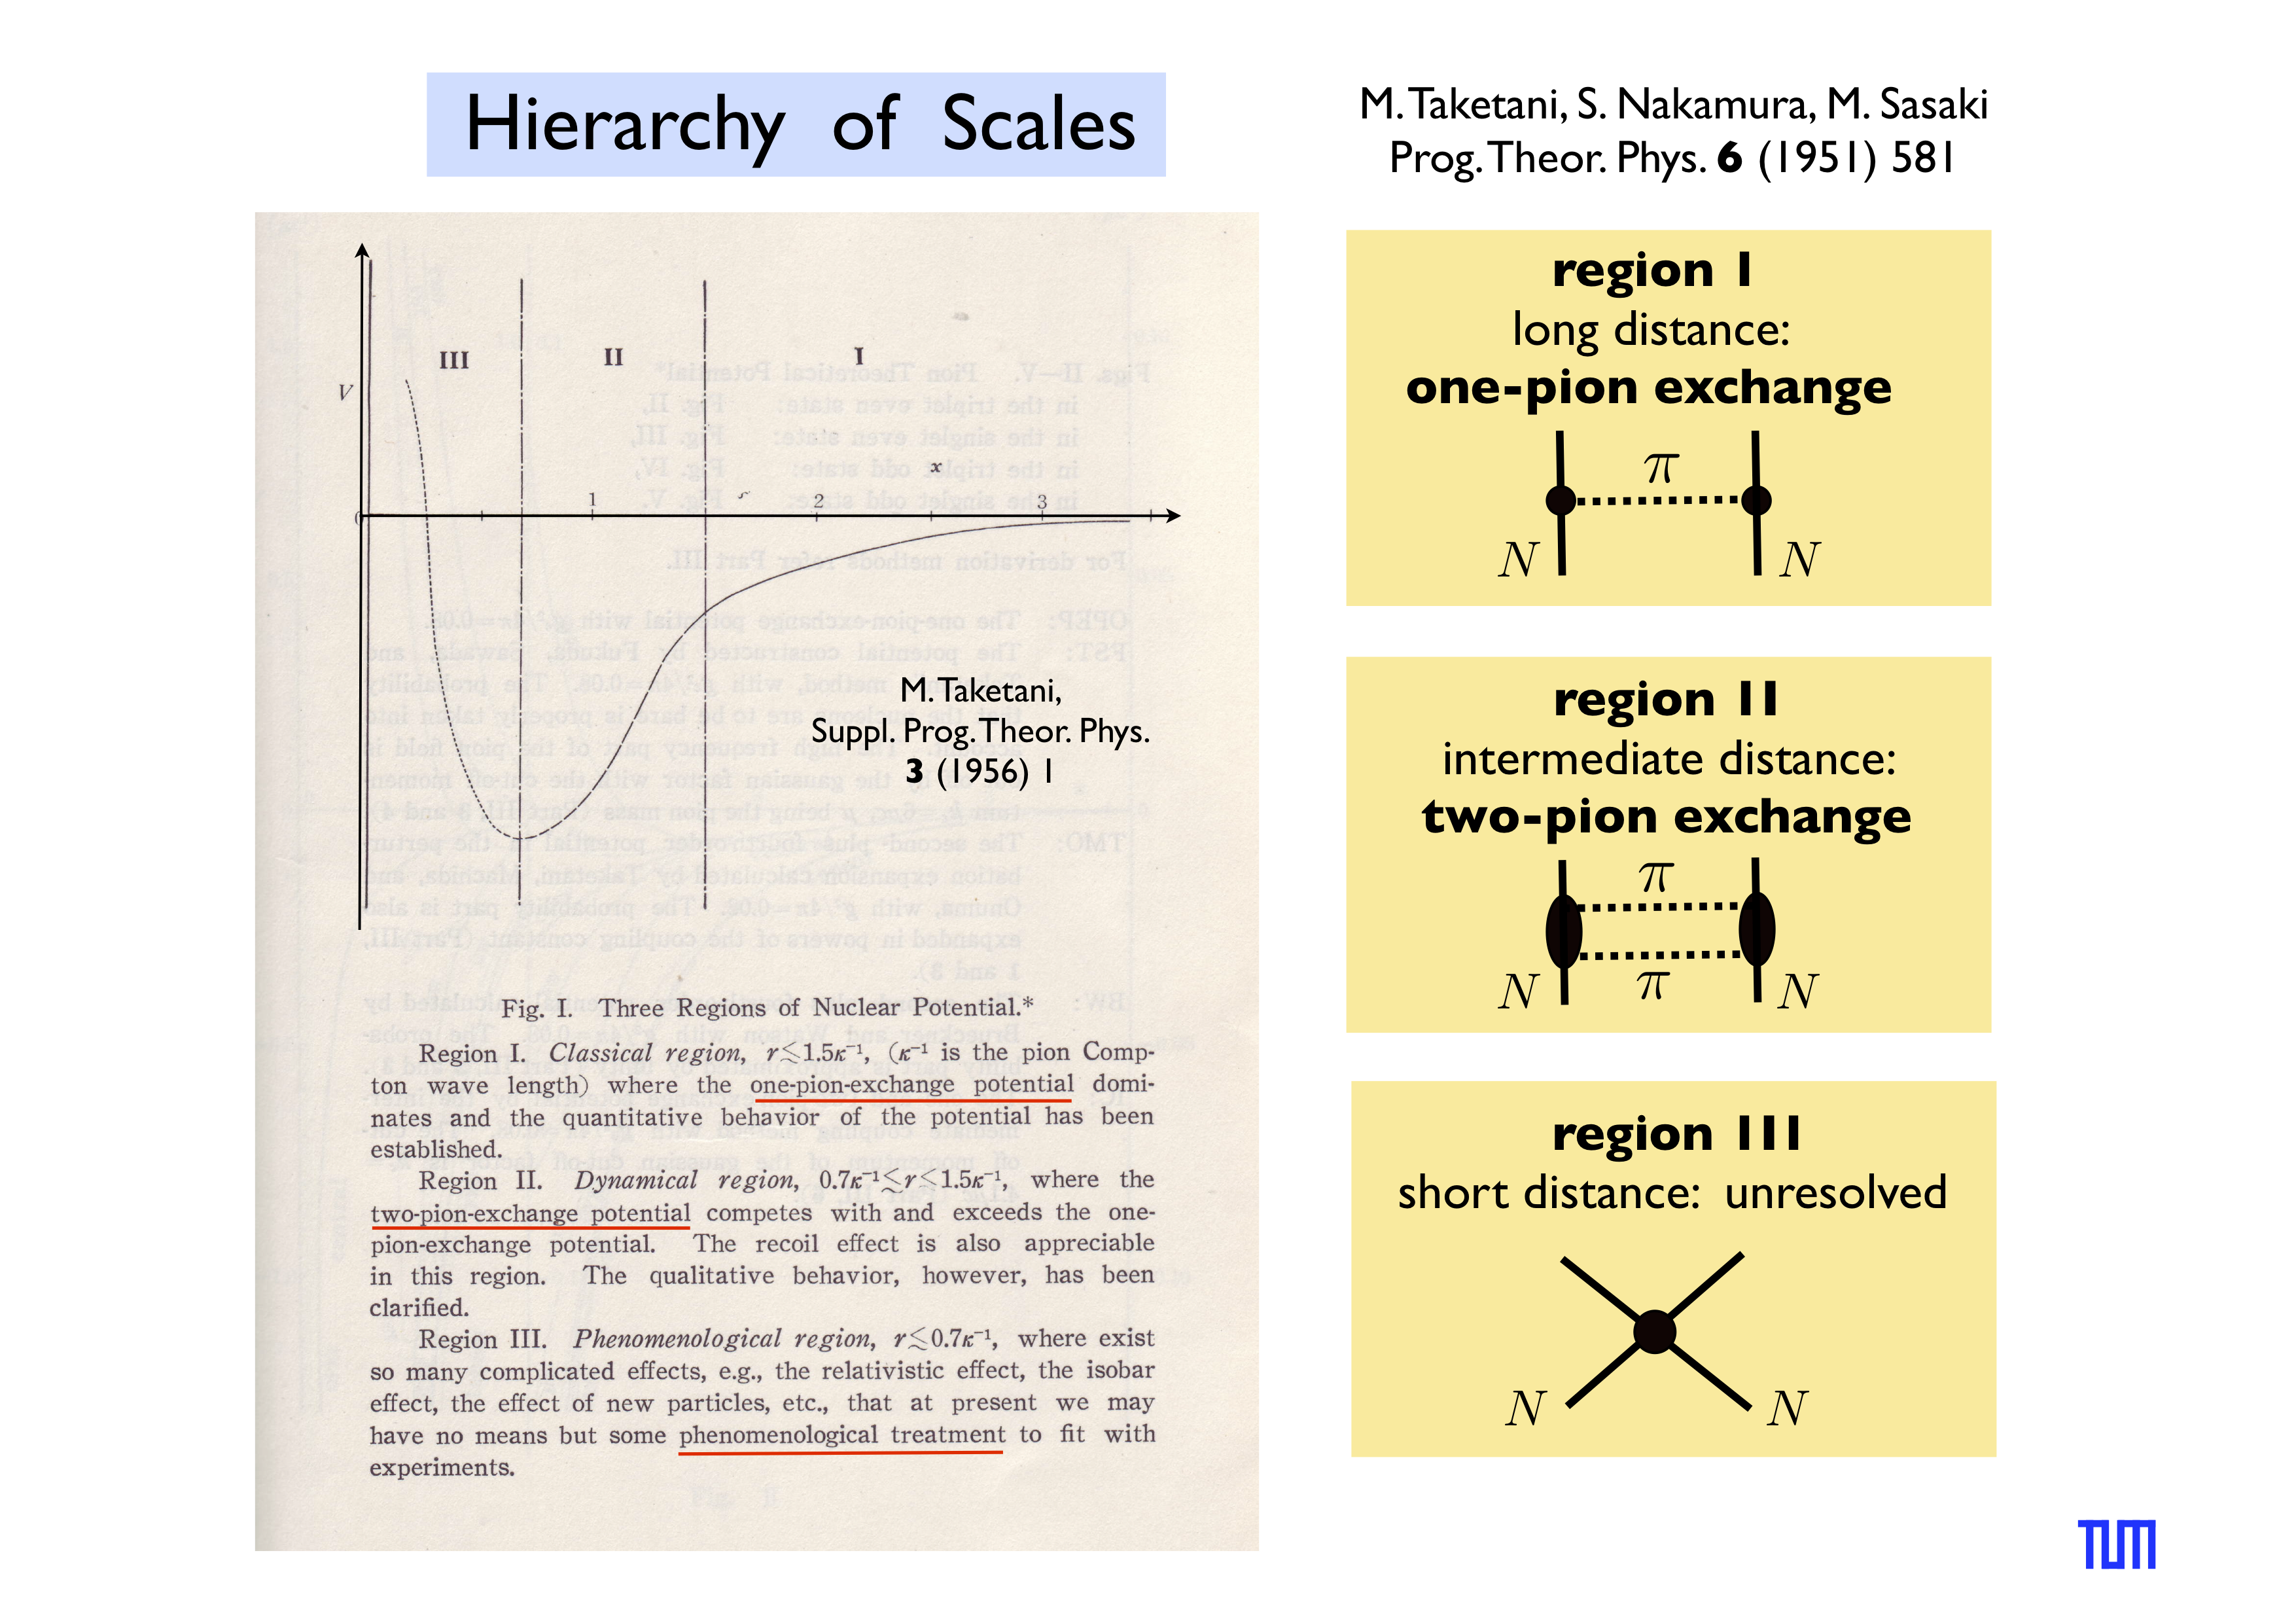
\includegraphics[width=\textwidth,height=(\textheight-11mm),keepaspectratio]{HSs}
\caption{Articolo di Taketani del 1956}
\label{fig:HSs}
\end{figure}



We can divide the region where the nuclear potential acts into three parts, taking the distance between two nucleons as a parameter, $x=\mu r$ con $\mu^{-1}$ lunghezza d'onda Compton del pione:
\begin{enumerate*}
\item Region I: r large. $x\geq1.5$.

The nuclear potential can be approximated by the static one-pion-exchange potential which is derived theoretically without any ambiguity.
\item Region II: Intermediate region. $0.7\geq x\geq1.5$.

We must take into account dynamical effects and the contribution from two-pion-exchange potential
\item Region III: short range, repulsive core. $x\leq0.7$.

QCD, exchange: many pions, strange particle. Relativistic effects
\end{enumerate*}


Nucleon-Nucleon interaction is always divided into three parts, as follows:
The NN potential is written as a sum of an electromagnetic (EM) part, a one-pion-exchange (OPE) part, and an intermediate- and short-range phenomenological part:
\begin{equation*}
V(NN)=V^{EM}(NN)+V^{\pi}(NN)+V^{R}(NN)
\end{equation*}
where
\begin{align*}
V^{\pi}(\Pproton\Pproton)=f^2_{pp}v_{\pi}(m_{\Ppizero})\\
V^{\pi}(\Pneutron\Pproton)=f_{pp}f_{nn}v_{\pi}(m_{\Ppizero})+(-)^{T+1}2f_c^2v_{\pi}(m_{\pi^{\pm}})\\
V^{\pi}(\Pneutron\Pneutron)=f^2_{nn}v_{\pi}(m_{\Ppizero})\\
\end{align*}
and
\begin{equation*}
v_{\pi}(m)=(\frac{m}{m_s})^2\frac{1}{3}mc^2[Y_{\mu}(r)\scap{\sigma_i}{\sigma_j}+T_{\mu}S_{ij}]
\end{equation*}
with
\begin{align*}
Y_{\mu}(r)=\frac{\exp{-\mu r}}{\mu r}(1-\exp{-cr^2}), \\
T_{\mu}(r)=(1+\frac{3}{\mu r}+\frac{3}{(\mu r)^2})\frac{\exp{-\mu r}}{\mu r}(1-\exp{-cr^2})^2
\end{align*}

The remaining intermediate and short-range phenomenological part of the potential is expressed, as in the Argonne $V_{14}$ model, as a sum of central, $L^2$, tensor, spin-orbit, and quadratic spin-orbit terms (abbreviated as $C$, $L_2$, $T$, $LS$, $LS^2$, respectively) in different $S$, $T$, and $T_3$, states.

\section{Potenziale TNS}

\subsection{Discovery of quadrupole electric moment of deuteron}
The original idea of a scalar field interacting with nucleon was soon extended to vectors and pseudo-vectors field:\\
the sign of quadrupole moment of deuteron was given correctly by exchange of (isovector) pseudoscalar meson (pion)


\subsection{strong pion-pion interaction}
Several phenomena dimonstrate a strong pion-pion interaction.

\subsection{Problem with 2 pions exchange}
Taketani, Nakamura, Sasaki proposed to subdivide the the range of nuclear force in 3 regions:

I classical long range  $r\geq2 fm$, II dynamical intermediate $1 fm< r <2 fm$, III core short range $r < 1 fm$.

Region I is dominated by OPE; region II by TPE (and heavier meson exchange); region III by multi-pion exchange heavy-meson and quark-gluon.

It's impossible to derive a sufficient  spin-orbit force from the 2\Pgp exchange: in 1960 Breit suggest to look for heavy vector boson in order to account short range spin-orbit force: $(\Pgr,\Pgo)$ was soon discovered.

\section{OBE}
Basic assumption:multi-pion exchange can be well accounted for by the exchange of multi-pion resonances, ie uncorrelated multi-pion exchange can be neglected.

\subsection{Other strongly interacting bosons}
I pioni sono i membri pi\'u leggeri della famiglia dei bosoni che risentono dell'interazione forte.

Gli altri sono \PK, \Peta, \Pgrp, \Pgo.


\section{Generalizzazione di Bethe}

\subsection{Laplaciano}

\begin{align*}
\nabla^2(\frac{1}{|\vec{r}-\vec{r_1}|})=-4\pi\delta^{(3)}(\vec{r}-\vec{r_1})
\end{align*}

\subsection{componenti potenziale NN}
\begin{align*}
V_{NN}=V_C{r}+V_{\sigma}(r)(\scap{\sigma_1}{\sigma_2})+V_T(r)S_{12}+\ldots\\
S_{12}=3\frac{(\scap{\sigma_1}{r})(\scap{\sigma_2}{r})}{r^2}-\scap{\sigma_1}{\sigma_2}
\end{align*}

\subsection{OPEP e la parit\'a del pione}
L'energia potenziale per il termine di sorgente $-g\delta^{(3)}(\vec{r}-\vec{r_0})$ \'e invariante per parit\'a (inversione spaziale)
\begin{equation*}
V(r)=g\phi(r)=\frac{g^2}{4\pi}\frac{\exp{-kr}}{r}
\end{equation*}
ma il pione ha parit\'a negativa quindi provo con un termine di sorgente diverso:

cio\'e tale che $\phi_{\pi}(-\vec{r})=-\phi(\vec{r})$.

\subsection{OPEP: generalizzazione di Bethe}
\begin{align*}
(\nabla^2-k_{\pi}^2)\phi_{\pi}(\vec{r})=-g(\scap{\sigma_1}{\nabla_1})\delta^{(3)}(\vec{r}-\vec{r_1})
\end{align*}
da cui
\begin{align*}
\phi_{\pi}(\vec{r})=\frac{g}{4\pi}(\scap{\sigma_1}{\nabla_1})\frac{\exp{-\frac{|\vec{r}-\vec{r_1}|}{\lambda_{\pi}}}}{|\vec{r}-\vec{r_1}|}
\end{align*}
e per l'energia potenziale 
\begin{align*}
V_{\pi}(\vec{r})=-\frac{g^2}{4\pi}(\scap{\sigma_1}{\nabla_1})\frac{\exp{-\frac{|\vec{r}-\vec{r_1}|}{\lambda_{\pi}}}}{|\vec{r}-\vec{r_1}|}
\end{align*}

\subsection{OPEP: forma esplicita}
\begin{align*}
V_{\pi}(\vec{r})&=-\frac{g^2}{4\pi}(\scap{\sigma_1}{\nabla_1})\frac{\exp{-\frac{|\vec{r}-\vec{r_1}|}{\lambda_{\pi}}}}{|\vec{r}-\vec{r_1}|}\\
&=-\frac{g^2}{4\pi}[\scap{\sigma_1}{\sigma_2}+(1+\frac{3\lambda_{\pi}}{r}+\frac{3\lambda_{\pi}}{r^2})S_{12}]\frac{\exp{-\frac{r}{\lambda_{\pi}}}}{r}\\
\end{align*}
in una forma pi\'u precisa
\begin{align*}
V_{\pi}(\vec{r})&=-\frac{1}{3}\frac{f^2}{4\pi}[\frac{\exp{-\frac{r}{\lambda_{\pi}}}}{r}-\frac{4\pi}{\mu^2}\delta^{(3)}(\vec{x})](\scap{\sigma_1}{\sigma_2})(\scap{\tau_1}{\tau_2})+\\
&-\frac{1}{3}\frac{f^2}{4\pi}[1+\frac{3}{\mu r}+\frac{3}{(\mu r)^2}]\frac{\exp{-\frac{r}{\lambda_{\pi}}}}{r}S_{12}(\hat{x})(\scap{\tau_1}{\tau_2})=\\
&=V_{\text{Scalar}}+V_{\text{Tensor}}
\end{align*}

\clearpage

\section{Teoria di Yukawa con mesoni di spin zero e oltre: il deutone}

\subsection{Analogia dipolo elettrico}

\subsection{Potential arising from pion exchange}
as non-relativistic limit of a $\gamma_5^{(1)}\cdot\gamma_5^{(2)}$ coupling of nucleons 1 and 2
\subsection{Laplacian identity}
$\nabla^2\frac{\exp{-k r}}{r}=k^2\frac{\exp{-kr}}{r}-4\pi\delta^{(3)}(\vec{x})$
\subsection{Fermi contact interaction}
\begin{equation*}
V_{em}=-\frac{1}{3}(\scap{d_1}{d_2})\delta^{(3)}(\vec{x})+\frac{d_1d_2}{4\pi}\frac{S_{12}(\hat{x})}{r^3}
\end{equation*}
evidente nella struttura iperfina degli spettri atomici.

\subsection{Point source of pionic field}
Starting from a non-relativistic $(\scap{\sigma}{\nabla})$ coupling:

for a point source at the origin of pion filed the source function is
\begin{equation*}
j^{\alpha}_{\pi}(\vec{x})=\frac{f}{\mu}\tau^{\alpha}(\scap{\sigma}{\nabla})\delta^{(3)}(\vec{x})
\end{equation*}
this is a dipole source emitting p-wave pions; the corrisponding pion field $\phi^{\alpha}(\vec{x})$ is\\
\begin{equation*}
\phi^{\alpha}(\vec{x})=-\frac{f}{\mu}\tau^{\alpha}(\scap{\sigma}{\nabla})\frac{\exp{-\mu r}}{r}
\end{equation*}
This pion field looks very much like the e.m. diploe field $\phi(\vec{x})$ outside a point dipole with dipole moment $\vec{d}$
\begin{equation*}
\phi(\vec{x})=-(\scap{d}{\nabla})\frac{1}{4\pi r}
\end{equation*}

Axial dipole moment associated with the nucleon creating pionic field.

It's usefull to associate an axial dipole moment
\begin{equation*}
\vec{m}^{\alpha}=(\frac{f}{\mu})\tau^{\alpha}\vec{\sigma}
\end{equation*}
 with the nucleon creating pionic field.

\begin{figure}[!ht]
\centering
\includegraphics[width=\textwidth,height=(\textheight-11mm),keepaspectratio]{pionic-em}
\caption{Analogy between electric Dipole-Dipole interaction and pionic Axial dipole-Axial dipole interaction}
\label{fig:pionic-em}
\end{figure}

\subsection{Pionic dipole-dipole interaction: Potential energy}
The corrisponding potential energy is the usual source-field coupling
\begin{equation*}
V_{\pi}=\int d^3xj_2^{\alpha}(\vec{x})\phi_1^{\alpha}(\vec{x})
\end{equation*}
which gives
\begin{equation*}
V_{\pi}=(\scap{\tau_1}{\tau_2})\frac{f^2}{\mu}(\scap{\sigma_1}{\nabla})(\scap{\sigma_2}{\nabla})\frac{\exp{-\mu r}}{4\pi r}
\end{equation*}
where $r=|\vec{x_1}-\vec{x_2}|$.
The above equation have identical structure of the em dipole-dipole interaction potential
\begin{equation*}
V_{em}=(\scap{d_1}{\nabla})\phi_1(\vec{x})=(\scap{d_1}{\nabla})(\scap{d_2}{\nabla})\frac{1}{4\pi r}
\end{equation*}

\section{Scambio di due pioni, forze nucleari a tre corpi Ruolo della particella $\Delta$ nella forza nucleare.}

\subsection{TPE - Risonanze}

$N_1$ emette 1 pione che va ad interagire con $N_2$ formando una risonanza $\Delta$, la quale decade rapidamente riemettendo un pione che interagisce con $N_1$.


\subsection{\Pgr-meson \Pgo-meson exchange}
Interazione mediata da risonanze \Pgr e \Pgo: core repulsivo

\lbt{m_{\Pgr}=770\Mcs}{m_{\Pgo}=783\Mcs} quindi stimo $R_{int}\approx\frac{\hbar c}{mc^2}\approx 0.2-0.5 fm$.

\subsection{Doppia interazione 2 corpi e a 3 corpi}

Doppia interazione a 2 corpi.
Interazioni a 3 corpi : risonananze $V_{123}$

\end{document}